%%
%%  AaltoTheses - LaTeX-tutkielmapohjat Aalto-tyylille
%%
%%  Hannu Tiitu
%%  hannu@tiitu.fi
%%
\begin{filecontents*}{\jobname.xmpdata}
  \Title{Evaluation of Managed Kubernetes Solutions for Enterprise Use-cases}
  \Author{Hung Vu}
  \Keywords{cloud native\sep distributed system \sep kubernetes \sep enterprise resource management}
  \Publisher{Aalto University}
\end{filecontents*}
\documentclass[oneside,pdfa,breaklinks]{aaltoseries}
\makeatletter
\@ifpackageloaded{inputenc}{%
  \inputencoding{utf8}}{%
  \usepackage[utf8]{inputenc}}
\hypersetup{hidelinks}              
\makeatother
\usepackage[finnish,english]{babel}   
\usepackage{setspace}                 % Rivivälin säätämiseksi
\usepackage{afterpage}                % Sivun taustaväri
\microtypesetup{letterspace=25}       % Kannen harvaan välistykseen

% My own packages
\usepackage{longtable}
\usepackage{amsmath}
\usepackage{url}
\def\UrlBreaks{\do\/\do-}
\usepackage{breakurl}
\usepackage{xpatch}
\usepackage{array}
\usepackage{booktabs}
% \usepackage[backend=bibtex,style=ieee,natbib=true]{biblatex}
% \usepackage[style=ieee,backend=biber]{biblatex}
\usepackage[
backend=biber,
sorting=none,
sortcites=true,
defernumbers=false,
bibstyle=ieee,
citestyle=numeric,
]{biblatex}
\AtEveryBibitem{
  \ifentrytype{online}
    {\clearfield{}}
    {\clearfield{url}
     \clearfield{urlyear}
     
    }  % Clear the url and access date fields for non-online entries
}
\xpatchbibdriver{online}
  {\printtext[parens]{\usebibmacro{date}}}
  {\iffieldundef{year}
    {}
    {\printtext[parens]{\usebibmacro{date}}}}
  {}
  {\typeout{There was an error patching biblatex-ieee (specifically, ieee.bbx's @online driver)}}
\addbibresource{references.bib}
\usepackage{xurl}
\usepackage{placeins}
\emergencystretch 3em



% My own definitions

\providecommand{\tightlist}{%
  \setlength{\itemsep}{0pt}\setlength{\parskip}{0pt}}

% Bibiography
% \bibliographystyle{IEEEtran}

% This is for highlighting %
\usepackage{xcolor}
\usepackage{soul}


\author{Hung Vu}
\title{Evaluation of Managed Kubernetes Solutions for Enterprise Use-cases}

\begin{document}



%%  KANSI  ---------------------------------------------

\thispagestyle{empty}
\setcounter{page}{0}  % Kansisivulle sivunumero 0

% Kansisivun marginaalit
\newgeometry{left=23.2mm,right=23.2mm,top=13.5mm,bottom=18mm}

% Punainen kansisivu
\pagecolor{aaltoRed}\afterpage{\nopagecolor}
{\color{black}  % Musta teksti

{\parindent0pt % Kappaleiden sisennys pois päältä
{\fontsize{11.9pt}{11.9pt}\bfseries\sffamily\lsstyle Bachelor’s Programme in Science and Technology}

\color{white}  % Valkoinen teksti alkaa

\vspace{13.1mm}

\begin{spacing}{3.1}
{\fontsize{35}{35}\selectfont Evaluation of Managed Kubernetes Solutions for Enterprise Use-cases}
\end{spacing}

\vspace{2.2mm}

\begin{spacing}{1.24}
{\fontsize{14pt}{14pt}\bfseries\sffamily\lsstyle }
\end{spacing}

\vspace{7.2mm}

\rule{\textwidth}{1.25pt}

\vspace{8.5mm}

{\fontsize{13.9pt}{13.9pt}\bfseries\sffamily\lsstyle Hung Vu}

\vfill

\begin{picture}(0,0)
\put(356,-7.8){\bfseries\sffamily\footnotesize\lsstyle BACHELOR'S}
\put(356,-17.4){\bfseries\sffamily\footnotesize\lsstyle THESIS}
\put(346,-26.5){\rule{.75pt}{25pt}}
\end{picture}

\AaltoLogoSmall{.66}{?}{white}

} % Kappaleiden sisennys takaisin käyttöön
} % Valkoisen tekstin pääätös



%%  NIMIÖSIVU  -----------------------------------------

\newpage

\pagenumbering{roman}

% Nimiösivun marginaalit
\newgeometry{left=80.7mm,right=25mm,top=12.9mm,bottom=21mm}
a
\thispagestyle{empty}

{\parindent0pt % Kappaleiden sisennys pois päältä
\begin{spacing}{1.1}
\hspace{-39.1mm}{\fontsize{10.5pt}{10.5pt}\sffamily\lsstyle Aalto University}

\hspace{-39.1mm}{\fontsize{10.5pt}{10.5pt}\bfseries\sffamily\lsstyle BACHELOR'S THESIS} {\sffamily\lsstyle 2024}
\end{spacing}

\vspace{12.7mm}

\begin{spacing}{1.63}
{\fontsize{17.8pt}{17.8pt}\selectfont Evaluation of Managed Kubernetes Solutions for Enterprise Use-cases}
\end{spacing}

\vspace{10.5mm}

\begin{spacing}{1.2}
{\fontsize{13pt}{13pt}\selectfont }
\end{spacing}

\vspace{10.6mm}

{\fontsize{13.9pt}{13.9pt}\bfseries\sffamily\lsstyle Hung Vu}

\vfill

{\fontsize{10.3pt}{10.3pt}\sffamily\lsstyle\raggedright
\begin{spacing}{1.06}

Thesis submitted in partial fulfilment of the requirements for the
degree of Bachelor of Science in Technology.

Otaniemi, 25 November 2024

\begin{tabbing}
Supervisor:\hspace{6mm} \= Prof. Gopika Premsankar (Aalto University) \\
Advisor: \> Mr. Daniel Tyrode (Nokia Oy)
\end{tabbing}
\vspace{-4mm}
\end{spacing}
} % fontsize

\vspace{11.5mm}

\begin{spacing}{.9}
{\bfseries\sffamily\lsstyle Aalto University \\
School of Science \\
Bachelor’s Programme in Science and Technology}
\end{spacing}
} % Kappaleiden sisennys takaisin käyttöön



%%  ABSTRACT  ------------------------------------------

\newpage
\phantomsection
\addcontentsline{toc}{chapter}{Abstract}

% Tiivistelmien marginaalit
\newgeometry{left=41.8mm,right=25mm,top=14.33mm,bottom=27mm}
% Alkuperäisessä Aalto-sarjassa marginaalit ovat suunnilleen näin:
%\newgeometry{left=41.8mm,right=17.6mm,top=14.33mm,bottom=20.4mm}

\begin{spacing}{.88}

{\parindent0pt % Kappaleiden sisennys pois päältä
\AaltoLogoSmall{.625}{''}{aaltoBlack}

{\fontsize{13.9pt}{13.9pt}\selectfont
\vspace{-8.9mm}\hfill{\bfseries\sffamily\lsstyle Abstract}}

{\fontsize{9.48pt}{9.48pt}\selectfont
\vspace{.9mm}\hfill{\bfseries\sffamily\lsstyle Aalto University, P.O. Box 11000, FI-00076 Aalto~~\textcolor{aaltoGray}{www.aalto.fi}}}

\vspace{7.8mm}{\fontsize{10.5pt}{10.5pt}\bfseries\sffamily\lsstyle Author}\\
{\small Hung Vu}

\vspace{-2.4mm}\rule{\textwidth}{.75pt}

{\fontsize{10.5pt}{10.5pt}\bfseries\sffamily\lsstyle Title}\\
\parbox[t]{\textwidth}{\raggedright\small Evaluation of Managed Kubernetes Solutions for Enterprise Use-cases}

\vspace{.5mm}\rule{\textwidth}{.75pt}

{\fontsize{10.5pt}{10.5pt}\bfseries\sffamily\lsstyle School}~~{\small School of Science}

\vspace{-2.4mm}\rule{\textwidth}{.75pt}

{\fontsize{10.5pt}{10.5pt}\bfseries\sffamily\lsstyle Degree programme}~~{\small Bachelor’s Programme in Science and Technology}

\vspace{-2.4mm}\rule{\textwidth}{.75pt}

{\fontsize{10.5pt}{10.5pt}\bfseries\sffamily\lsstyle Major}~~{\small Digital Systems and Design}\hfill{\fontsize{10.5pt}{10.5pt}\bfseries\sffamily\lsstyle Code}~~{\small (unknown)}

\vspace{-2.4mm}\rule{\textwidth}{.75pt}

{\fontsize{10.5pt}{10.5pt}\bfseries\sffamily\lsstyle Supervisor}~~{\small Prof. Gopika Premsankar (Aalto University)}

\vspace{-2.4mm}\rule{\textwidth}{.75pt}

{\fontsize{10.5pt}{10.5pt}\bfseries\sffamily\lsstyle Advisor}~~{\small Mr. Daniel Tyrode (Nokia Oy)}

\vspace{-2.4mm}\rule{\textwidth}{.75pt}

{\fontsize{10.5pt}{10.5pt}\bfseries\sffamily\lsstyle Level}~~{\small Bachelor's thesis}\hfill{\fontsize{10.5pt}{10.5pt}\bfseries\sffamily\lsstyle Date}~~{\small 31 May 2024}\hfill{\fontsize{10.5pt}{10.5pt}\bfseries\sffamily\lsstyle Pages}~~{\small 70}\hfill{\fontsize{10.5pt}{10.5pt}\bfseries\sffamily\lsstyle Language}~~{\small English}

\vspace{-2.4mm}\rule{\textwidth}{.75pt}

\vspace{6mm}

} % Kappaleiden sisennys takaisin käyttöön
\end{spacing}
\begin{spacing}{1.05}

\noindent{\fontsize{10.5pt}{10.5pt}\bfseries\sffamily\lsstyle Abstract}
\vspace{.8mm}

{\small
  Abstract here (not required in the research plan)
}

\vfill

\end{spacing}
\begin{spacing}{.88}
{\parindent0pt % Kappaleiden sisennys pois päältä

\makebox[19mm][l]{\fontsize{10.5pt}{10.5pt}\bfseries\sffamily\lsstyle Keywords}\parbox[t]{123.6mm}{\raggedright\small cloud native, distributed systems, kubernetes, enterprise resource management}

\vspace{.5mm}\rule{\textwidth}{.75pt}

{\fontsize{10.5pt}{10.5pt}\bfseries\sffamily\lsstyle urn}~~{\small https://aaltodoc.aalto.fi}

\vspace{-2.4mm}\rule{\textwidth}{.75pt}

} % Kappaleiden sisennys takaisin käyttöön
\end{spacing}



%%  TIIVISTELMÄ  ---------------------------------------

% \newpage
% \phantomsection
% \addcontentsline{toc}{chapter}{Tiivistelmä}

% % Tiivistelmäsivu suomeksi
% \selectlanguage{finnish}

% \begin{spacing}{.88}

% {\parindent0pt % Kappaleiden sisennys pois päältä
% \AaltoLogoSmall{.625}{!}{aaltoBlack}

% {\fontsize{13.9pt}{13.9pt}\selectfont
% \vspace{-8.9mm}\hfill{\bfseries\sffamily\lsstyle Tiivistelmä}}

% {\fontsize{9.48pt}{9.48pt}\selectfont
% \vspace{.9mm}\hfill{\bfseries\sffamily\lsstyle Aalto-yliopisto, PL 11000, 00076 Aalto~~\textcolor{aaltoGray}{www.aalto.fi}}}

% \vspace{7.8mm}{\fontsize{10.5pt}{10.5pt}\bfseries\sffamily\lsstyle Tekijä}\\
% {\small Hung Vu}

% \vspace{-2.4mm}\rule{\textwidth}{.75pt}

% {\fontsize{10.5pt}{10.5pt}\bfseries\sffamily\lsstyle Työn nimi}\\
% \parbox[t]{\textwidth}{\raggedright\small Oikeisiin virheisiin! Virheelliset vastaukset ja niiden tulkinta automaattisesti tarkastetuissa matematiikan harjoitustehtävissä}

% \vspace{.5mm}\rule{\textwidth}{.75pt}

% {\fontsize{10.5pt}{10.5pt}\bfseries\sffamily\lsstyle Korkeakoulu}~~{\small Perustieteiden korkeakoulu}

% \vspace{-2.4mm}\rule{\textwidth}{.75pt}

% {\fontsize{10.5pt}{10.5pt}\bfseries\sffamily\lsstyle Koulutusohjelma}~~{\small Teknistieteellinen kandidaattiohjelma}

% \vspace{-2.4mm}\rule{\textwidth}{.75pt}

% {\fontsize{10.5pt}{10.5pt}\bfseries\sffamily\lsstyle Pääaine}~~{\small Mediatekniikka}\hfill{\fontsize{10.5pt}{10.5pt}\bfseries\sffamily\lsstyle Koodi}~~{\small IL3011}

% \vspace{-2.4mm}\rule{\textwidth}{.75pt}

% {\fontsize{10.5pt}{10.5pt}\bfseries\sffamily\lsstyle Vastuuopettaja}~~{\small professori Lauri Malmi}

% \vspace{-2.4mm}\rule{\textwidth}{.75pt}

% {\fontsize{10.5pt}{10.5pt}\bfseries\sffamily\lsstyle Ohjaaja}~~{\small dosentti Jarmo Malinen}

% \vspace{-2.4mm}\rule{\textwidth}{.75pt}

% {\fontsize{10.5pt}{10.5pt}\bfseries\sffamily\lsstyle Työn laji}~~{\small Kandidaatintyö}\hfill{\fontsize{10.5pt}{10.5pt}\bfseries\sffamily\lsstyle Päiväys}~~{\small 27.11.2017}\hfill{\fontsize{10.5pt}{10.5pt}\bfseries\sffamily\lsstyle Sivuja}~~{\small 70}\hfill{\fontsize{10.5pt}{10.5pt}\bfseries\sffamily\lsstyle Kieli}~~{\small englanti}

% \vspace{-2.4mm}\rule{\textwidth}{.75pt}

% \vspace{6mm}

% } % Kappaleiden sisennys takaisin käyttöön
% \end{spacing}
% \begin{spacing}{1.05}

% \noindent{\fontsize{10.5pt}{10.5pt}\bfseries\sffamily\lsstyle Tiivistelmä}
% \vspace{.8mm}

% {\small
%   Lorem ipsum dolor sit amet, consectetuer adipiscing elit. Ut purus
%   elit, vestibulum ut, placerat ac, adipiscing vitae, felis. Curabitur
%   dictum gravida mauris. Nam arcu libero, nonummy eget, consectetuer
%   id, vulputate a, magna. Donec vehicula augue eu neque. Pellentesque
%   habitant morbi tristique senectus et netus et malesuada fames ac
%   turpis egestas. Mauris ut leo. Cras viverra metus rhoncus sem. Nulla
%   et lectus vestibulum urna fringilla ultrices. Phasellus eu tellus
%   sit amet tortor gravida placerat. Integer sapien est, iaculis in,
%   pretium quis, viverra ac, nunc. Praesent eget sem vel leo ultrices
%   bibendum. Aenean faucibus. Morbi dolor nulla, malesuada eu, pulvinar
%   at, mollis ac, nulla. Curabitur auctor semper nulla.  Donec varius
%   orci eget risus. Duis nibh mi, congue eu, accumsan eleifend,
%   sagittis quis, diam. Duis eget orci sit amet orci dignissim rutrum.

%   Nam dui ligula, fringilla a, euismod sodales, sollicitudin vel,
%   wisi. Morbi auctor lorem non justo. Nam lacus libero, pretium at,
%   lobortis vitae, ultricies et, tellus. Donec aliquet, tortor sed
%   accumsan bibendum, erat ligula aliquet magna, vitae ornare odio
%   metus a mi. Morbi ac orci et nisl hendrerit mollis. Suspendisse ut
%   massa. Cras nec ante. Pellentesque a nulla.  Cum sociis natoque
%   penatibus et magnis dis parturient montes, nascetur ridiculus
%   mus. Aliquam tincidunt urna. Nulla ullamcorper vestibulum
%   turpis. Pellentesque cursus luctus mauris.

%   Nulla malesuada porttitor diam. Donec felis erat, congue non,
%   volutpat at, tincidunt tristique, libero. Vivamus viverra fermentum
%   felis. Donec nonummy pellentesque ante. Phasellus adipiscing semper
%   elit. Proin fermentum massa ac quam. Sed diam turpis, molestie
%   vitae, placerat a, molestie nec, leo. Maecenas lacinia. Nam ipsum
%   ligula, eleifend at, accumsan nec, suscipit a, ipsum. Morbi blandit
%   ligula feugiat magna. Nunc eleifend consequat lorem. Sed lacinia
%   nulla vitae enim. Pellentesque tincidunt purus vel magna. Integer
%   non enim. Praesent euismod nunc eu purus.  Donec bibendum quam in
%   tellus. Nullam cursus pulvinar lectus. Donec et mi. Nam vulputate
%   metus eu enim. Vestibulum pellentesque felis eu massa.
% }

% \vfill

% \end{spacing}
% \begin{spacing}{.88}
% {\parindent0pt % Kappaleiden sisennys pois päältä

% \makebox[21mm][l]{\fontsize{10.5pt}{10.5pt}\bfseries\sffamily\lsstyle Avainsanat}\parbox[t]{121.6mm}{\raggedright\small oppimisympäristö, pedagoginen käytettävyys, virheluokittelu, automaattinen tarkastaminen, matematiikan opetus, Stack}

% \vspace{.5mm}\rule{\textwidth}{.75pt}

% {\fontsize{10.5pt}{10.5pt}\bfseries\sffamily\lsstyle urn}~~{\small https://aaltodoc.aalto.fi}

% \vspace{-2.4mm}\rule{\textwidth}{.75pt}

% } % Kappaleiden sisennys takaisin käyttöön
% \end{spacing}

% \selectlanguage{english}  % Palataan englantiin
% \restoregeometry  % Palataan normaaleihin sivumarginaaleihin



%%  SISÄLTÖ  -------------------------------------------

\newpage

\tableofcontents

%%  TYÖ ALKAA TÄSTÄ  -----------------------------------

\newpage

\pagenumbering{arabic}

\chapter{Introduction}

The cloud is a concept that was first introduced in 2006 with the launch of the first public cloud service (Simple Storage Service, S3 on the 13th of March 2006) \cite{liuReviewDigitalTwin2021}. Since then, the field has experienced rapid growth and development, with the rise of various tools, frameworks, and paradigms. Notably, a core technology that characterises modern cloud computing is \textit{containerisation} \cite{pereiraferreiraPerformanceEvaluationContainers2019}. Through containerisation, application dependencies can be packaged in “containers” that share access to the underlying host OS kernel, allowing multiple containers with different dependencies to be hosted on the same hardware.

While being resource-efficient, the adoption of containers in the cloud faces a new set of challenges in terms of automation, scalability, and management \cite{pereiraferreiraPerformanceEvaluationContainers2019}. To address these challenges, a range of container orchestration tools were developed. The most notable being Kubernetes, an open-source container orchestration platform that was originally developed by Google \cite{Kubernetes, pereiraferreiraPerformanceEvaluationContainers2019}. Although other tools such as Docker Swarm exist, Kubernetes remains as the industry’s de facto standard in terms of container management due to its robust reliability, extensive feature set, and broad ecosystem \cite{truyenComprehensiveFeatureComparison2019}.

Kubernetes can manage hundreds of thousands of containers, making it extremely scalable. In addition to the upstream Kubernetes, various Kubernetes distributions were developed to cater towards specific use-cases, such as edge computing and enterprise environments. In managed Kubernetes for enterprise use-cases in particular, the focus is on providing features like streamlined application deployment, enhanced security, advanced management capability, and optimised resource utilisation for large-scale applications \cite{WhatEnterpriseKubernetes, truyenComprehensiveFeatureComparison2019, jiangIndustrialApplicationsDigital2021}. This combination of scalability and enhanced functionality makes managed Kubernetes a preferred choice for organisations over native Kubernetes and other open-source alternatives \cite{redhatinc.StateKubernetesSecurity2024, vrabicDigitalTwinsUnderstanding2018, portworxKubernetesAdoptionSurvey2021, broadcomStateKubernetes20232023}.

With the ever-growing demand for managed Kubernetes distribution at the enterprise level, multiple service providers such as Amazon, Microsoft, Google, Red Hat, and VMware, all offer their own flavour of Kubernetes (EKS, GKE, AKS, OpenShift, and VMware Tanzu respectively) \cite{AmazonEKSCustomers, maEurekaHumanLevelReward2023, nickomangAzureKubernetesService, redhatinc.RedHatOpenShift, VMwareTanzuPlatform}. Each distribution has its pros and cons, but they all offer a high degree of feature availability that elevates Kubernetes beyond its upstream version with tools for monitoring, scaling, managing, and securing enterprise workloads.

In addition to their varying feature sets, these distributions also differ in terms of their cost structure, which can be further broken down into infrastructure, management, and additional service costs. 

Although Kubernetes distributions' performance are relatively well-researched, few studies look at the managed Kubernetes distributions in terms of features and cost of operation \cite{bohmProfilingLightweightContainer2021, kjorveziroskiKubernetesDistributionsEdge2022, ascensaoAssessingKubernetesDistributions2024, pereiraferreiraPerformanceEvaluationContainers2019}. These aspects, especially the cost, are crucial for companies and organisations to make informed decision on their distribution of choice.

Therefore, this thesis aims to identify the current state of Kubernetes adoption and key challenges to derive key feature requirements for Kubernetes distributions. Based on these requirements, it then compares various distributions and evaluates their ability to address said requirements, as well as the expected cost of operation for each distribution. The goal of this work is to provide a comprehensive assessment of available managed Kubernetes offerings and identify the best-suited options for the industry to meet the most common set of requirements.

Among managed Kubernetes distributions, EKS, GKE, AKS, and OpenShift consistently rank among the most widely adopted distributions for organisations \cite{redhatinc.StateKubernetesSecurity2024, canonicalKubernetesCloudNative2022, portworxKubernetesAdoptionSurvey2021, broadcomStateKubernetes20232023}. Thus, these four distributions are chosen for assessment to make the work relevant to Nokia and the industry at large. The evaluation consists of three main parts: a brief literature review on the current state of managed Kubernetes distributions, a feature comparison, and a cost analysis for the selected distributions.

The subsequent sections of this thesis are arranged as follows. Section 2 provides background on the relevant technologies to Kubernetes and the mentioned managed Kubernetes distributions. Section 3 outlines the research methodology. Section 4 compiles and interprets results from the review. Lastly, Section 5 concludes the findings and discusses potential topics for further research.

% \section{Fusce mauris}

% Fusce mauris. Vestibulum luctus nibh at lectus. Sed bibendum, nulla a
% faucibus semper, leo velit ultricies tellus, ac venenatis arcu wisi
% vel nisl.  Vestibulum diam. Aliquam pellentesque, augue quis sagittis
% posuere, turpis lacus congue quam, in hendrerit risus eros eget
% felis. Maecenas eget erat in sapien mattis porttitor. Vestibulum
% porttitor. Nulla facilisi.  Sed a turpis eu lacus commodo
% facilisis. Morbi fringilla, wisi in dignissim interdum, justo lectus
% sagittis dui, et vehicula libero dui cursus dui. Mauris tempor ligula
% sed lacus. Duis cursus enim ut augue. Cras ac magna.  Cras
% nulla. Nulla egestas. Curabitur a leo. Quisque egestas wisi eget
% nunc. Nam feugiat lacus vel est. Curabitur consectetuer.

% Suspendisse vel felis. Ut lorem lorem, interdum eu, tincidunt sit
% amet, laoreet vitae, arcu. Aenean faucibus pede eu ante. Praesent enim
% elit, rutrum at, molestie non, nonummy vel, nisl. Ut lectus eros,
% malesuada sit amet, fermentum eu, sodales cursus, magna. Donec eu
% purus. Quisque vehicula, urna sed ultricies auctor, pede lorem egestas
% dui, et convallis elit erat sed nulla. Donec luctus. Curabitur et
% nunc. Aliquam dolor odio, commodo pretium, ultricies non, pharetra in,
% velit. Integer arcu est, nonummy in, fermentum faucibus, egestas vel,
% odio.

% \subsection{Sed commodo posuere pede}

% Sed commodo posuere pede. Mauris ut est. Ut quis purus. Sed ac odio.
% Sed vehicula hendrerit sem. Duis non odio. Morbi ut dui. Sed accumsan
% risus eget odio. In hac habitasse platea dictumst. Pellentesque non
% elit.  Fusce sed justo eu urna porta tincidunt. Mauris felis odio,
% sollicitudin sed, volutpat a, ornare ac, erat. Morbi quis dolor. Donec
% pellentesque, erat ac sagittis semper, nunc dui lobortis purus, quis
% congue purus metus ultricies tellus. Proin et quam. Class aptent
% taciti sociosqu ad litora torquent per conubia nostra, per inceptos
% hymenaeos. Praesent sapien turpis, fermentum vel, eleifend faucibus,
% vehicula eu, lacus.

% Pellentesque habitant morbi tristique senectus et netus et malesuada
% fames ac turpis egestas. Donec odio elit, dictum in, hendrerit sit
% amet, egestas sed, leo. Praesent feugiat sapien aliquet odio. Integer
% vitae justo.  Aliquam vestibulum fringilla lorem. Sed neque lectus,
% consectetuer at, consectetuer sed, eleifend ac, lectus. Nulla
% facilisi. Pellentesque eget lectus. Proin eu metus. Sed porttitor. In
% hac habitasse platea dictumst. Suspendisse eu lectus. Ut mi mi,
% lacinia sit amet, placerat et, mollis vitae, dui. Sed ante tellus,
% tristique ut, iaculis eu, malesuada ac, dui. Mauris nibh leo,
% facilisis non, adipiscing quis, ultrices a, dui.

% \subsection{Morbi luctus}

% Morbi luctus, wisi viverra faucibus pretium, nibh est placerat odio,
% nec commodo wisi enim eget quam. Quisque libero justo, consectetuer a,
% feugiat vitae, porttitor eu, libero. Suspendisse sed mauris vitae elit
% sollicitudin malesuada. Maecenas ultricies eros sit amet ante. Ut
% venenatis velit. Maecenas sed mi eget dui varius euismod. Phasellus
% aliquet volutpat odio. Vestibulum ante ipsum primis in faucibus orci
% luctus et ultrices posuere cubilia Curae; Pellentesque sit amet pede
% ac sem eleifend consectetuer. Nullam elementum, urna vel imperdiet
% sodales, elit ipsum pharetra ligula, ac pretium ante justo a
% nulla. Curabitur tristique arcu eu metus. Vestibulum lectus. Proin
% mauris. Proin eu nunc eu urna hendrerit faucibus. Aliquam auctor, pede
% consequat laoreet varius, eros tellus scelerisque quam, pellentesque
% hendrerit ipsum dolor sed augue. Nulla nec lacus.

% Suspendisse vitae elit. Aliquam arcu neque, ornare in, ullamcorper
% quis, commodo eu, libero. Fusce sagittis erat at erat tristique
% mollis. Maecenas sapien libero, molestie et, lobortis in, sodales
% eget, dui. Morbi ultrices rutrum lorem. Nam elementum ullamcorper
% leo. Morbi dui. Aliquam sagittis. Nunc placerat. Pellentesque
% tristique sodales est. Maecenas imperdiet lacinia velit. Cras non
% urna. Morbi eros pede, suscipit ac, varius vel, egestas non,
% eros. Praesent malesuada, diam id pretium elementum, eros sem dictum
% tortor, vel consectetuer odio sem sed wisi.

% \section{Sed feugiat}

% Sed feugiat. Cum sociis natoque penatibus et magnis dis parturient
% montes, nascetur ridiculus mus. Ut pellentesque augue sed
% urna. Vestibulum diam eros, fringilla et, consectetuer eu, nonummy id,
% sapien. Nullam at lectus. In sagittis ultrices mauris. Curabitur
% malesuada erat sit amet massa. Fusce blandit. Aliquam erat
% volutpat. Aliquam euismod. Aenean vel lectus. Nunc imperdiet justo nec
% dolor.

% Etiam euismod. Fusce facilisis lacinia dui. Suspendisse potenti. In mi
% erat, cursus id, nonummy sed, ullamcorper eget, sapien. Praesent
% pretium, magna in eleifend egestas, pede pede pretium lorem, quis
% consectetuer tortor sapien facilisis magna. Mauris quis magna varius
% nulla scelerisque imperdiet. Aliquam non quam. Aliquam porttitor quam
% a lacus.  Praesent vel arcu ut tortor cursus volutpat. In vitae pede
% quis diam bibendum placerat. Fusce elementum convallis neque. Sed
% dolor orci, scelerisque ac, dapibus nec, ultricies ut, mi. Duis nec
% dui quis leo sagittis commodo.


\chapter{Background}

- Go through some of the definitions (i.e. what are contested, what are agreed upon)\\
- Explain certain concepts such as Kubernetes and cloud-native\\
- Explain what the managed Kubernetes solutions are\\
- Explain what OpenShift HyperShift is and brief architectural discussion (compare with the architecture of the public cloud Kubernetes solutions)\\

\section{The Cloud}

Cloud computing is a paradigm that enables companies to utilise computing resources over the internet without the need to manage infrastructure directly. According to the US National Institute of Standards and Technology, the cloud facilitates "ubiquitous, convenient, on-demand network access to a shared pool of configurable computing resources (e.g., networks, servers, storage, applications, and services) that can be rapidly provisioned and released with minimal management effort or service provider interaction" \cite{editorCloudComputingGlossary}. This offers businesses significant flexibility, scalability, and cost savings. Cloud services can be divided into three primary deployment models: Public Cloud, Private Cloud, and Hybrid Cloud \cite{ramgovind2010management}.

\subsection{Public Cloud}

In recent years, public cloud appears to be the most commonly adopted deployment model \cite{VoiceKubernetesExperts,CNCFAnnualSurvey2024, opara2016critical}. At the time of writing, the leading public cloud providers are Amazon, Microsoft, and Google \cite{2024StateCloud}. In this model, organisations can rent necessary resources based on their usage from a shared pool. This allows organisations to utilise cloud resources without investing in physical infrastructure upfront. Furthermore, public cloud also offers tenants the ability to elastically adjust resource levels according to demand, scaling up or down as needed to potentially reduce costs \cite{suleiman2012understanding}. Public clouds are also traditionally considered less secure than other cloud models due to being hosted off-premise by third-party vendors \cite{sakr2011survey}. However, the security risk can be mitigated with appropriate countermeasure \cite{fox2009above}.


\subsection{Private Cloud}

In a private cloud setup, organisations obtain dedicated cloud environments exclusively for their usage. In contrast with the public cloud, a private cloud ensures isolation of infrastructure and services, offering enhanced control, customisation, and security. Private clouds are often hosted on-premise. This dedicated environment can be tailored to meet the specific needs of the organisation \cite{ramgovind2010management}.

\subsection{Hybrid Cloud}

A hybrid cloud deployment allows users to access features from both private and public clouds, taking advantage of both environments \cite{ramgovind2010management, dash2016governance}. This model allows organisations to run sensitive or critical workloads in-house, while leveraging the public cloud for less sensitive tasks. In addition, the integration of public cloud into the deployment also accommodates scaling requirements during peak demand, thus letting organisations optimise for both security and cost-efficiency \cite{huangAchievingBigData2014}.




\section{Vitualisation}

The cloud has evolved a lot since the beginning. However, one concept that remains crucial for cloud computing is virtualisation. Virtualisation enables the hosting of multiple software packages on the same physical hardware. This is achieved by allowing applications to access \textit{virtualised} hardware to utilise for their computational needs \cite{goldbergSurveyVirtualMachine1974}.

One widely used technique for virtualisation in computing is Virtual Machines (VMs), which aims to replicate computer systems on a processor instruction-basis. Each VM has its own operating system with processor instructions and system resources such as memory and I/O capabilities. These virtualised hardware compartments are made available to the VM by an abstraction layer called the hypervisor. The hypervisor is situated between the VM's operating system (guest OS) and the server's operating system (host OS), providing the guest OS access to the server's hardware. This setup enables multiple VMs to operate on the same server simultaneously \cite{goldbergSurveyVirtualMachine1974}.

This capability promotes operations such as software testing, application isolation, and system management. In addition, each VM is designed to function independently without disruptions from other virtual instances, thus improving the overall reliability and security of the entire system. \cite{goldbergSurveyVirtualMachine1974}.

Despite the aforementioned benefits of VMs regarding isolation and reliability, replicating an operating system in full requires additional computation overhead. This was one of the challenges that \textit{containers} aim to solve. Containers are portable software packages that include not only the application(s), but also all the necessary components (e.g. libraries and binaries) to run said application(s) \cite{bernsteinContainersCloudLXC2014}. Thanks to this, containers can, similar to VMs, ensures consistent operation across various environments, regardless of the underlying hardware and operating system.

The key differences between the two methods of virtualisation lies in the way they access the underlying hardware of the server. In contrast to Virtual Machines, which requires a distinct operating system for each instance, containers utilise the kernel of the host OS to execute instructions. This design allows containers to be more resource-efficient and faster to deploy, while still ensuring a degree of isolation between processes. These advantages make containers a favourable choice for cloud environments in the recent years, where scalability, performance, and resource efficiency are crucial requirements \cite{bernsteinContainersCloudLXC2014, felterUpdatedPerformanceComparison2015}.

\begin{figure}
    \centering
    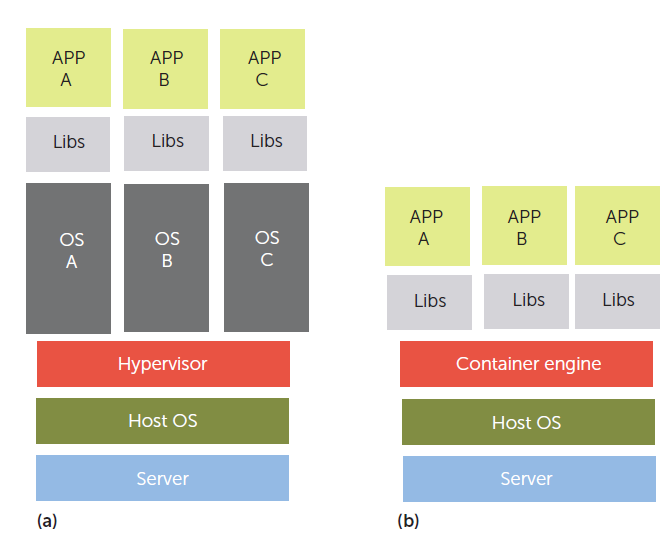
\includegraphics[width=0.7\linewidth]{resources/eea3da004befcc5437960cbc868be634.png}
    \caption{Architectural comparison of (a) virtual machine and (b) container \cite{bernsteinContainersCloudLXC2014}}
    \label{fig:vms-vs-containers}
\end{figure}

\section{Container Orchestration}

As the number of concurrently running containers grows, managing them quickly becomes challenging. Therefore, some form of automation is required to ease this orchestration process at scale. This is precisely the issue that container orchestration (CO) tools aim to solve. Similar to an orchestrator for an orchestra, CO technologies ensure that distributed containers work together harmoniously. By employing OC frameworks, enterprises and organisations can improve how resources are allocated, as well as simplify how they manage containers in cloud native settings \cite{truyenComprehensiveFeatureComparison2019}.

CO frameworks such as Kubernetes and Docker Swarm effectively manage the deployment, scaling, and networking of containers across multiple machines, allowing said machines to form clusters. These clusters are interconnected computers act as unified computing units that can handle containerised workloads, offloading the management responsibilities (connectivity, workload scheduling, scaling, resource allocation, etc.) from application developers \cite{Nodes, UsingMinikubeCreate}. In other words, from the developer's perspective, the cluster can be treated as a single computing unit to schedule workload. This configuration allows containerised applications to be distributed across multiple nodes in a straightforward manner. The design pattern is known as \textit{distributed application}, which is one of the most common design pattern in cloud computing due to its scalability and resiliency \cite{fehling2014cloud,kratzkeUnderstandingCloudnativeApplications2017}.

CO platforms compliment these benefits of distributed and containerised applications by minimising the management overhead, reducing the complexity of maintaining such configuration. The importance of workload distribution and containerisation in cloud infrastructure combine with the added benefits of CO platforms make them an important topic for research in both academia and industry. This focus on CO platforms and cloud-native application principles was revealed to be the research topic that gathered the most attention in a 2017 study \cite{kratzkeUnderstandingCloudnativeApplications2017}. The cloud space has evolved a lot since then. However, CO platforms still play a central role in today's cloud. The prevelant of CO platforms can be seen from the popularity of Kubernetes as a project, which will be discussed in section \ref{kubernetes}


\section{Cloud-native}
There are a variety of components that constitute a cloud-native application. However, as proposed by Gannon et al. \cite{gannonCloudNativeApplications2017}, cloud-native applications are designed to take advantage of the cloud environment. This entails utilising the fluid and distributed nature of the cloud to provide services that can operate at a global scale with low latency and high reliability \cite{gannonCloudNativeApplications2017}.

The Cloud-Native Computing Foundation (CNCF), part of the Linux Foundation, is an organisation that seeks to drive forward the cloud-native technologies and practices. They are the leading body in terms of setting best-practices recommendations in the cloud-native space. Many of the projects that they support, such as Kubernetes, Prometheus, HELM, and ArgoCD become de facto tools for cloud-native application development, monitoring, orchestration, and deployment. CNCF defined cloud-native as technologies that enable the development and deployment of scalable applications in cloud environments \cite{cloudnativecomputingfoundationWhoWeAre}. The application could be hosted on public, private, or hybrid cloud. However, in order to support the previously mentioned requirements, they usually possess the following attributes:

\begin{enumerate}
\item
  \textbf{Containers}: Compact, self-sufficient units containing all necessary components to run software, promoting uniformity from development through to deployment.
\item
  \textbf{Service Meshes}: Infrastructure layer that facilitates direct and manageable communication within microservices setups, enhancing clarity and control over service interactions.
\item
  \textbf{Microservices}: Design philosophy that organises applications into a network of small, independent services, each fulfilling a specific atomic function.
\item
  \textbf{Immutable Infrastructure}: Method that involves renewing or reconstructing infrastructure elements instead of modifying them, aiming to minimise discrepancies and prevent failures.
\item
  \textbf{Declarative APIs}: Interfaces that enable developers to define their requirements explicitly without detailing the execution process, streamlining application oversight by hiding the complexity of the underlying operations.
\end{enumerate}

\section{Kubernetes}\label{kubernetes}
\subsection{Background}

Developed by Google and later donated to the CNCF, Kubernetes is an open-source CO platform for automating the deployment, scaling, and operation of application containers \cite{Kubernetes}. Currently, it is one of the most popular cloud-native technologies with over 111,000 stars on GitHub, and has been accepted as the industry standard for container orchestration \cite{truyenComprehensiveFeatureComparison2019, KubernetesKubernetesProductionGrade}. It's specifically built to scale — capable of orchestrating thousands of containers across multiple environments (public, private and hybrid clouds).

Kubernetes offers several key features that make it well-suited for cloud-native application management:

\begin{itemize}

\item \textbf{Automated Scheduling}: Container placement in a cluster is done by automatically scheduling workloads considering resource availability and constraints to maximize infrastructure efficiency. 

\item \textbf{Self-Healing}: Kubernetes monitors the health of containers and nodes in the cluster and attempt to recover them in case of failures through initiating restart or rescheduling tasks.

\item \textbf{Horizontal Scaling}: Applications can adjust the number of container instances based on real-time demand automatically or manually in response to specified metric(s).

\item \textbf{Service discovery and load balancing}: Service discovery is simplified via the use of DNS names or IP addresses, with the network traffic being evenly distributed among container.

\item \textbf{Storage Orchestration}: Containers can have storage set up that is handled automatically with a wide variety of options including local storage, cloud-provisioned storage, and network file systems.

\item \textbf{Secret and Configuration Management}: Kubernetes handle sensitive data such as passwords, tokens, and configuration details and ensure that only the designated containers have access to them. 

\end{itemize}

In addition to its core functionality, Kubernetes has fostered a diverse portfolio of supportive tools and services such as Helm for package management, Prometheus for monitoring purposes, and ArgoCD for continuous delivery \cite{Helm, prometheusOverviewPrometheus, ArgoCDDeclarative}. This ecosystem plays a significant role in solidifying Kubernetes' central position in the modern cloud-native landscape.

\subsection{Distributions}
As a widely adopted tool across various industry, it is impossible for the upstream Kubernetes distribution to cater to all the different requirements and use-cases of its user. Thus, different Kubernetes \textit{distributions} emerged to address these specific needs, such as light-weight deployment and managed deployment \cite{bohmProfilingLightweightContainer2021, pereiraferreiraPerformanceEvaluationContainers2019}. From the licensing and management perspective, Kubernetes distributions largely falls into two categories: open-source (self-managed) and proprietary (managed).

\subsubsection{Open-source Kubernetes Distributions}

For organisations that prioritise flexibility, one potential option is to adopt an open-source Kubernetes distribution. Due to the lack of standards, there are certain differences between cloud service providers. According to Truyen et al. \cite{truyenManagingFeatureCompatibility2020}, these discrepancies largely fall into the following groups: cluster architecture and setup; framework customization interfaces; and feature incompatibilities. The disparity between vendors can create compatibility challenges when the need for platform migration arises. Open-source solutions' main strength is mitigating the risk of vendor lock-in \cite{shaikh2011total}. The differences will be discussed in further detail in the Related Works section.

\subsubsection{Managed Kubernetes Distributions}

Despite the high degree of customisability and flexibility that the open-source solutions offer, they lack the advanced features that managed Kubernetes distributions offer. Some of these features could include, for instance, automate control plane management (updating and maintaining Kubernetes control plane)l; cluster auto-scaling (scaling the underlying collection of compute nodes according to demand); and Kubelet configuration API (Kubelet configurations can be done through an API instead of through command-line parameters) \cite{truyenManagingFeatureCompatibility2020, KubeletConfigMachineconfigurationopenshiftioV1, AmazonEKSCustomers, RedHatOpenShiftb}. As a result, there is a significant disparity in adoption, with organisations favouring managed solutions over open-source ones \cite{redhatinc.StateKubernetesSecurity2024}.

\paragraph{Managed Kubernetes in the Cloud}\mbox{}

In the context of managed Kubernetes, some major public cloud options are Amazon Elastic Kubernetes Service (EKS), Google Kubernetes Engine (GKE), Azure Kubernetes Service (AKS), Red Hat OpenShift \footnote{At the time of writing, OpenShift offer 5 public cloud provider options for cloud-hosted infrastructure: AWS, Azure, Google, and IBM \cite{OpenShiftContainerPlatform}}, and VMware Tanzu \cite{AmazonEKSCustomers, maEurekaHumanLevelReward2023, nickomangAzureKubernetesService, redhatinc.RedHatOpenShift, VMwareTanzuPlatform}.

This thesis focuses strictly on public cloud managed Kubernetes offerings, due to the limited availability of pricing information for the self-managed/private cloud option. For instance, Red Hat OpenShift \cite{redhatinc.RedHatOpenShift}. In addition, as mentioned in the section on Public Cloud, it is the most common cloud deployment model. Pereira et al. \cite{pereiraferreiraPerformanceEvaluationContainers2019} suggested that this is true for Kubernetes hosting preference as well, with cloud-hosted Kubernetes becoming more common. In the paper, this was attributed to the auto-provisioning (or auto-scaling) capability, along with the management aid that cloud-hosted Kubernetes offers.

\section{Interest in Kubernetes and Managed Kubernetes}

\subsection{Google Trends}

\FloatBarrier  

\begin{figure}
    \centering
    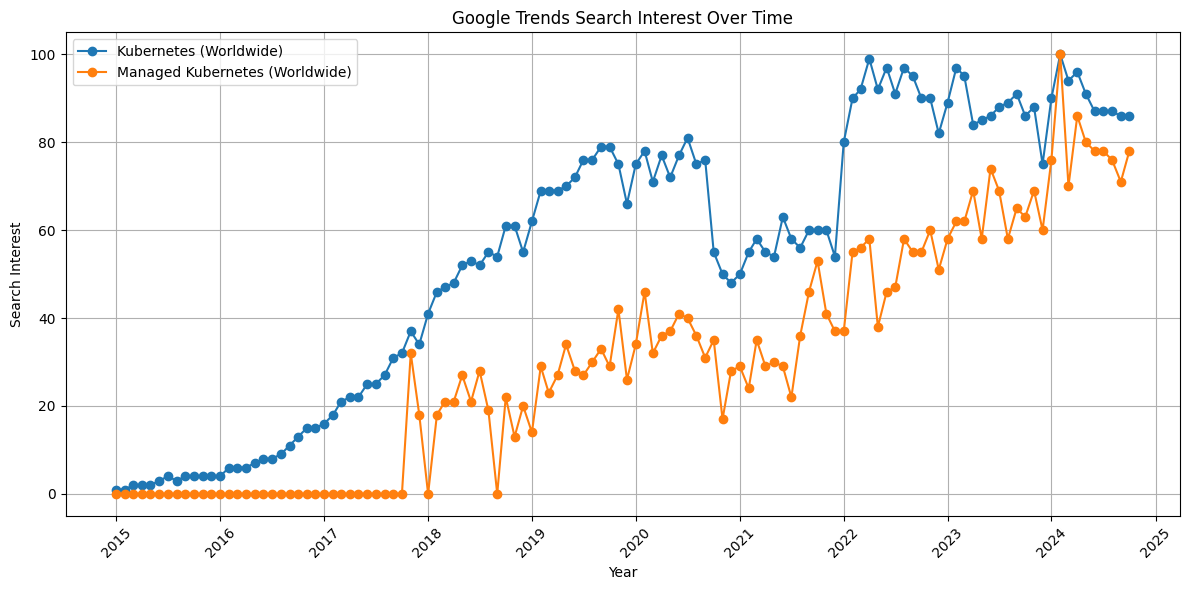
\includegraphics[width=1\linewidth]{resources/d2a89eeeda76d50039bc6f5d3a97c41b.png}
    \caption{Google Trends search interest in Kubernetes vs managed Kubernetes}
    \label{fig:search-interests-kubernetes-vs-managed-kubernetes}
\end{figure}

To provide context for the topic covered in this thesis, this section looks at the popularity of Kubernetes and managed Kubernetes by examining Google Trends search data and the yearly publications data from the Web of Science database. Kratzke et al. proposed that Google Trend can serve as a resource for spotting “industrial buzzwords” and new trends in the technology sector \cite{kratzkeUnderstandingCloudnativeApplications2017}. By combining this data with an analysis of research publications, we can gain insights into evolving trends in both the industry and in academia. The keywords examined are “Kubernetes” and “managed Kubernetes” (case-insensitive) and the timeframe spans from the earliest data-point to October 2024, which is one month prior to the completion of this thesis.

The graph depicted in Figure \ref{fig:search-interests-kubernetes-vs-managed-kubernetes} shows the search interest on Google for “Kubernetes” compared to “managed Kubernetes”. From the plot, it can be discerned that there is a steady rise in popularity for Kubernetes since its introduction until the peak around 2022, after which the search interest stabilises.

One noteworthy aspect is the drop in search activity observed in 2021; however, the reason behind this decline remains ambiguous. Similar search trends were observed for various cloud-native technologies such as Docker and Fluentd, showing comparable decreases. This commonality suggests that although the root cause remains unknown, this change may have influenced a wide array of adjacent technologies in the cloud-native sphere.

The Google Trends data also highlights a convergence in interest for Kubernetes and managed Kubernetes, especially in recent years. The growing preference for managed Kubernetes could indicate a rising awareness among users and businesses about the benefits of managed solutions.

The preference for managed Kubernetes is further supported through industrial reports and surveys. For instance, a 2022 report by Canonical indicated that only 19.3\% of respondents use native (self-managed) Kubernetes \cite{canonicalKubernetesCloudNative2022}. Similarly, Red Hat's 2024 state of Kubernetes security report showed comparable data, with just 23\% of respondents using self-managed Kubernetes \cite{redhatinc.StateKubernetesSecurity2024}.

\subsection{Research Publications}

\FloatBarrier

\begin{figure}
    \centering
    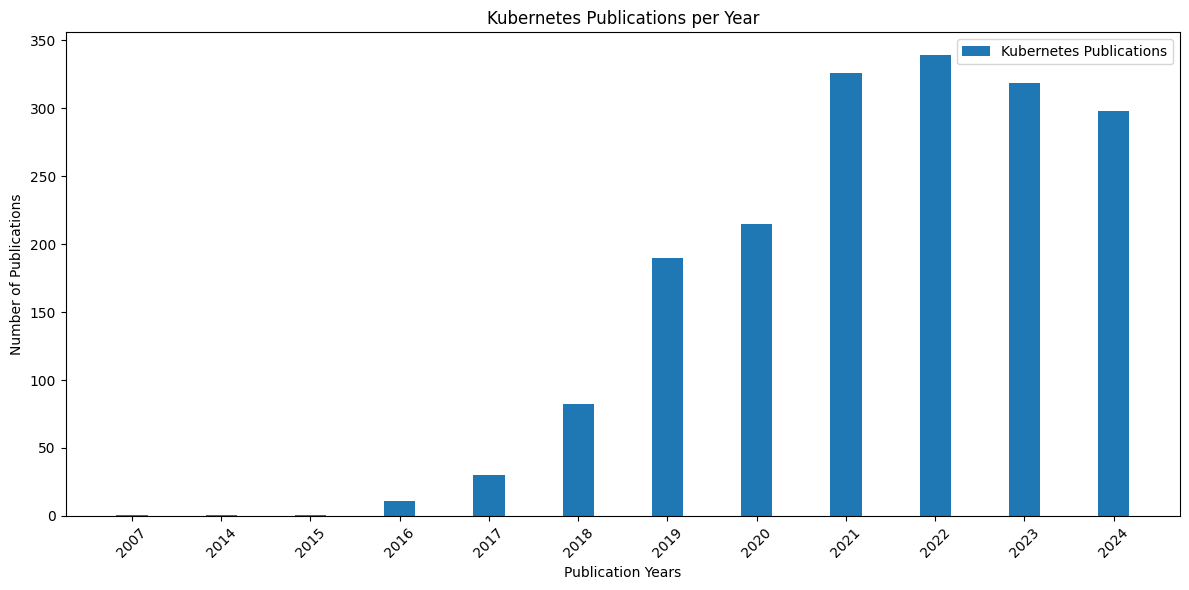
\includegraphics[width=1\linewidth]{resources/publications-plot-k8s.png}
    \caption{Annual Research Publications on Kubernetes}
    \label{fig:research-publications-kubernetes-and-managed-kubernetes}
\end{figure}


\begin{figure}
    \centering
    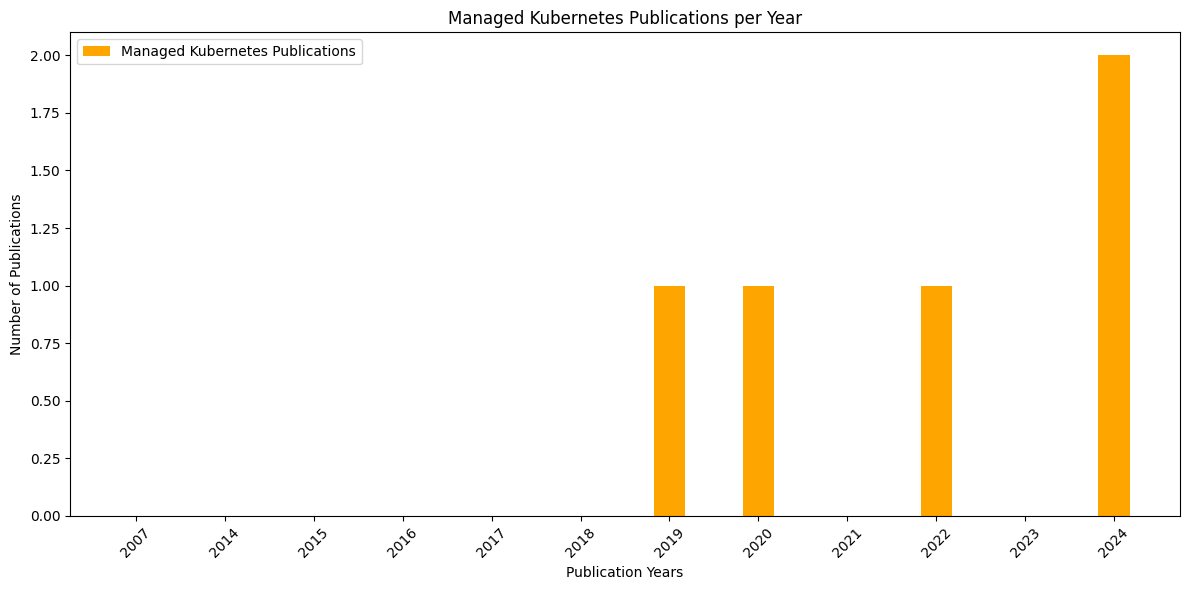
\includegraphics[width=1\linewidth]{resources/publications-plot-managed-k8s.png}
    \caption{Annual Research Publications on Managed Kubernetes}
    \label{fig:research-publications-managed-kubernetes}
\end{figure}

This process of analysing academic interest for the given topics involved collecting information on the yearly publication count through the Web of Science result analysis tool. This annual publication data, shown in Figure \ref{fig:research-publications-kubernetes-and-managed-kubernetes}, reflects a steady increase in Kubernetes-related publications until the peak in 2022. This trends aligns with the results demonstrated by the Google Trends data.

The term 'managed Kubernetes' was chosen because it appears to be a common term for distributions such as AKS, EKS, GKE, and OCP \cite{AmazonEKSCustomers,ManagedKubernetesService,pereiraferreiraPerformanceEvaluationContainers2019}. However, as depicted by the plot in Figure \ref{fig:research-publications-managed-kubernetes} above, the number of hits for 'managed Kubernetes' was surprisingly low. In order to widen the scope of the search, the following query was used to capture all mentions of these distributions in the topic: \texttt{`TS=((EKS OR "Elastic Kubernetes Service" OR AKS OR "Azure Kubernetes Service" OR GKE OR "Google Kubernetes Engine" OR OCP OR "OpenShift Container Platform" OR "managed kubernetes") AND "kubernetes")`}. This query matches all results with any of the managed Kubernetes distribution mentioned in the Title, Abstract, or Keyword. In addition, it filters out any results that \textit{do not} contain "Kubernetes". This aims to avoid irrelevant matches from other fields (for example, medical and biology) that are unrelated to the current search.

Plotting the results again, it can be observed that although the number of matches has increased compared to the previous query with \texttt{"managed kubernetes"}. However, the number of publications remains at a modest amount from 2019 to 2023. On the other hand, there seems to be a spike in the number of publications in 2024. It is unclear whether this is a temporary increase or the start of a long-term trend in managed Kubernetes research.

\FloatBarrier


\begin{figure}
    \centering
    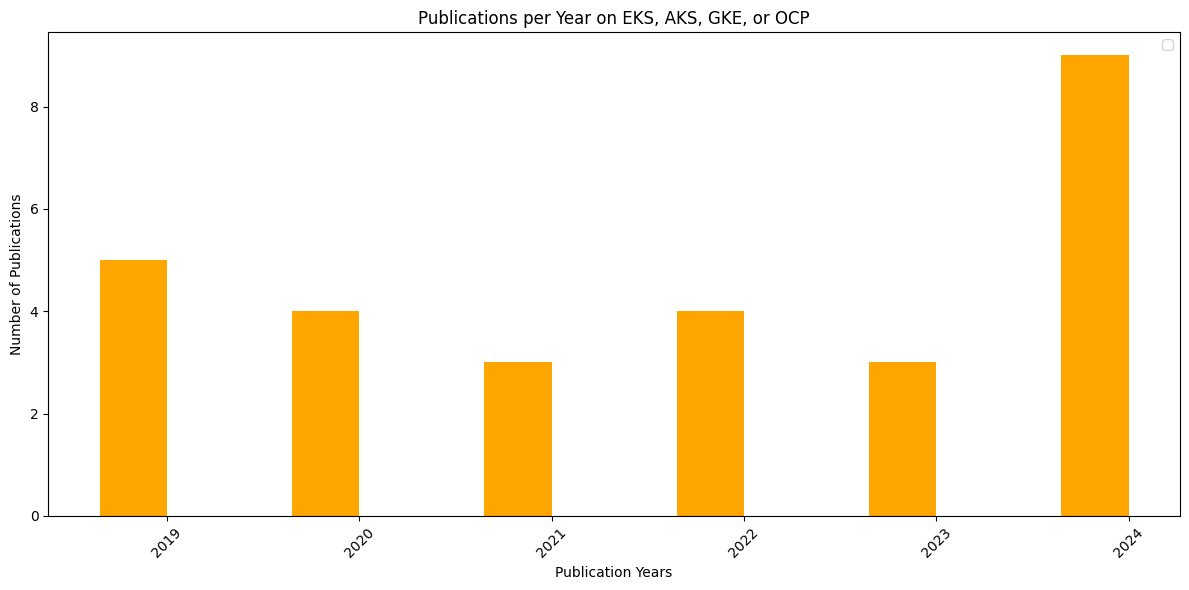
\includegraphics[width=1\linewidth]{resources/managed-k8s-broaden-scope.png}
    \caption{Annual Research Publications on the managed Kubernetes examined (EKS, AKS, GKE, OCP)}
    \label{fig:managed-k8s-broaden-scope}
\end{figure}


Nevertheless, it is worth noting that managed Kubernetes has not received the same level of attention in academic research as it has in Google Trends. There was only a rather limited number of publications annually from 2019 to 2024. As observed by Bunse et al. \cite{BUNSE2011667}, there could be potential research gaps between what the industry needs and what has been researched by available scientific literatures. Given the available data, it could be possible that despite growing interests, "managed Kubernetes" is not getting the adequate research focus. This disparity indicates that there could be potential for further academic investigation into managed Kubernetes (e.g. features, performance, and costs), similar to Ferreira’s study \cite{pereiraferreiraPerformanceEvaluationContainers2019}.

Regarding the observed peak in publications for "Kubernetes", a 2019 study by Truyen et al. \cite{truyenComprehensiveFeatureComparison2019} proposed that container orchestration technologies were entering the peak of the Gartner hype cycle. However, both the Google Trends data and the number of annually published articles seem to suggest otherwise. From these insights, it appears that Kubernetes likely reached its peak in popularity around 2022.

These statistics indicate a rising interest in both Kubernetes and managed Kubernetes, highlighting the relevance of the thesis topic. The increasing interest in managed Kubernetes, combined with the lack of research evaluating managed Kubernetes solutions, demonstrated a potential for further academic exploration and analysis to address this gap. With the focus on examining the most suitable managed Kubernetes distribution, the thesis falls under the "best of breed" stream of research. It was mentioned by Marston et al. \cite{MARSTON2011176} that this research stream is a highly relevant vein of research for cloud-computing.

\section{Related Works}
\subsubsection{Differences Between K8s vendors and vendor lock-in}
Truyen et al \cite{truyenManagingFeatureCompatibility2020} look at three major Kubernetes distributions (EKS, AKS, GKE) and compare them in terms of feature compatibility and potential of vendor lock-in. The main groups of differences proposed are:

\begin{itemize}

\item \textbf{Architectural}: Differences in terms of the way the platform is implemented. For example, the operating system choice of the platform.
\item \textbf{Customization interfaces}: Differences in terms of how Kubernetes components can be configured. For example, the Container Network Interface (CNI) choices that the distribution provide (Calico, Cilium, Flannel, etc.)
\item \textbf{Feature incompatibilities}: Differences in terms of feature availability. This could be in the form of API resources, Custom Resource Definitions (CRDs), etc. For example, the SCC custom resource is only available on OCP.

\end{itemize}

These divergences can bring migration challenges, which introduces a risk called \textit{vendor lock-in}. Vendor lock-in happens when an organisation becomes dependent on a product, while alternative options require significant efforts (e.g. costs, technical, legal) \cite{opara2016critical}.

\subsubsection{Ease of Migration Analysis}

Due to the mentioned differences between platforms, migrating from one platform to another can prove to be a challenging procedure. Truyen et al. \cite{cloudnativecomputingfoundationFrequentlyAskedQuestions2018} evaluated AKS, EKS, and GKE in terms of pair-wise migratability mapping across these differences. 

The paper discussed potential errors in the recorded findings due to some test results being inconsistent with the official documentation. After adjusting for these errors, EKS possesses the lowest number of incompatible occurrences, making it the most configurable distribution out of the ones examined. In other words, when strictly considering their compatibility with native Kubernetes' customisation interfaces, EKS is more compatible than the other two vendors \textit{after potential configurations}.

GKE, on the other hand, has the highest number of Kubernetes features that work \textit{out-of-the-box}. This means that out-of-the-box with zero configuration, GKE is the most compatible with native Kubernetes' feature set, making it the more feature-rich distribution.

In short, EKS is more compatible when taking into account potential configuration steps, while GKE is more compatible while taking into account the out-of-the-box state of the distribution.

The work shown that there are non-negligible differences even among major players in the managed Kubernetes space and the compatibility between evaluated platforms. However, the paper did not assess the importance of the features provided by the platforms as well as the differences in cost of operation. In addition, OCP was not evaluated in the study. As one of the most popular managed Kubernetes distributions, there are potential valuable insights that can be obtained from examining OCP and comparing it against other offerings \cite{redhatinc.StateKubernetesSecurity2024, vrabicDigitalTwinsUnderstanding2018, portworxKubernetesAdoptionSurvey2021, broadcomStateKubernetes20232023}.


\subsubsection{Performance analysis of managed Kubernetes distributions}

In a 2019 paper, Pereira et al. \cite{pereiraferreiraPerformanceEvaluationContainers2019} evaluated the three major managed Kubernetes distributions (EKS, AKS, and GKE) in terms of performance. The performance evaluation is characterised by four key computing characteristics: CPU, memory, disk, and network. To obtain a baseline for these metrics, the paper made use of the performance of the NeCTAR Research Cloud.

The findings suggested that there is no definitive "best" solution that outperforms on all metrics examined. However, it was observed that EKS outperform the others on CPU, memory, and disk I/O benchmarks, while GKE possesses superior performance on the network benchmark \cite{pereiraferreiraPerformanceEvaluationContainers2019}.

Similar to the Truyen et al. paper \cite{truyenManagingFeatureCompatibility2020}, the paper did not include OCP in the evaluation, and did not include an analysis on feature and costs. However, it was noted that the related costs to the scaling operations of these services could be a potential area to study in the future \cite{pereiraferreiraPerformanceEvaluationContainers2019}.

As mentioned in the paper, as well as demonstrated by the number of yearly publications above, the literature covering the performance of these managed solutions is rather sparse. Open-source Kubernetes distributions, on the other hand, have received significantly more attention in terms of research \cite{bohmProfilingLightweightContainer2021,koziolekLightweightKubernetesDistributions2023,ascensaoAssessingKubernetesDistributions2024,9660392,bryantKubernetesDeploymentOptions2024}. Given the high degree of variations amongst the managed distributions in terms of performance, features, and costs, further research could provide valuable insights that aid organisations in making informed decisions on their distribution of choice.

\subsubsection{Feature Analysis}

To the best of our knowledge, the most similar study to this thesis is a recent 2024 article by Kumar et al. \cite{10499108}. The paper examined different cloud container technologies, including EKS, GKE, AKS, and Red Hat OpenShift, amongts with other platforms and technologies. It compares the platforms in terms of features such as maximum number of nodes, security method, storage provisioning method etc. Additionally, a rough cost comparison of the services was also provided.

Kumar et al. \cite{10499108} provided a thorough analysis of the similarities, as well as the differences, between the Kubernetes platforms examined. Nevertheless, the work provided a general comparison of the platforms in order to provide complementary insights for users to aid in decision-making. Therefore, the comparison is provided in general terms. For instance, in contrasts to the Truyen et al. paper \cite{truyenManagingFeatureCompatibility2020}, the cluster installation time is given in terms such as "Takes time" and "Easy installation". While these insights are useful for evaluating suitable platforms for organisational needs, they are too vague to systematically determine what platform is best or most suitable. In other words, it is challenging to grade and rank the technologies simply based on these qualitative statements.

This thesis will focuses on evaluating relevant features for enterprises (as identified in the Evaluation Criteria section) in a quantifiable manner. From the evaluation results, it is possible to identify of what the most suitable managed Kubernetes distribution is, given the established criteria and parameters. However, the methodology can be adopted and customised to case-by-case requirements by modifying those variables. This enables users to perform a multi-criteria appraisal and determine the most appropriate distribution based on their organisation's needs.

\chapter{Evaluation Criteria}\label{chap:evaluation-criteria}

\section{Key Feature}

The core research question examined in this thesis is "What is the most suitable managed Kubernetes distribution for enterprise?" In order to answer this question, we must first define what constitute a “suitable” distribution for enterprise use-cases. In other words, what are the most important factors for company and organisations when adopting a Kubernetes platform. Towards this end, five major industrial report in the timeframe 2022-2024 were reviewed. From each report, three top challenges adopting Kubernetes or cloud-native platforms are identified. The findings can be found from table \ref{tab:challenges-from-surveys}.


\begin{tiny} 
\begin{longtable}{|p{0.2\linewidth}|p{0.3\linewidth}|p{0.45\linewidth}|} % Adjusted column widths
\hline
\textbf{Source} & \textbf{Question} & \textbf{Top Challenges} \\
\hline
Portworx 2022 Annual Kubernetes Adoption Report \cite{2022AnnualKubernetes} & What are the challenges that are the most difficult to overcome when running Kubernetes (ranked top three)? & 
\raggedright 1. Security \newline 2. Data management \newline 3. Reliability \tabularnewline
\hline
Broadcom State of Cloud Native App Platforms 2024 Report \cite{StateCloudNative} & What challenges do organizations encounter in building or adopting a cloud native app platform? & 
\raggedright 1. Meeting compliance and security requirements \newline 2. Integration with existing data sources and repositories \newline 3. Distributed ownership deployment and management \tabularnewline
\hline
Canonical Kubernetes and Cloud Native Operations Report 2022 \cite{canonicalKubernetesCloudNative2022} & What are the top challenges Kubernetes brings to businesses? & 
\raggedright 1. Security and compliance concerns not addressed adequately \newline 2. Integrating cloud-native applications together \newline 3. Poor or limited support from platform providers or partners \tabularnewline
\hline
Spectrocloud 2024 State of Production Kubernetes Survey \cite{2024StateProduction} & What challenges does your organization face with running Kubernetes in production? & 
\raggedright 1. It’s difficult to choose and validate the right stack components from the broad cloud-native ecosystem \newline 2. Configuration drift causes issues with compliance and availability \newline 3. We struggle to properly protect ourselves against security breaches \tabularnewline
\hline
CNCF Annual Survey 2023 \cite{CNCFAnnualSurvey2024} & What are your Challenges in Using / Deploying Containers? & 
\raggedright 1. Security \newline 2. Complexity \newline 3. Monitoring \tabularnewline
\hline
\caption{Challenges from Various Surveys} \label{tab:challenges-from-surveys} \\
\end{longtable}
\end{tiny}
From these insights, it is clear that security is the most pressing concern for organisations. Therefore, security features are selected as the key indicator of distribution suitability in this thesis. However, it is worth noting that this evaluation criteria can be changed for future evaluation depending on the requirements of the respective organisation.

\section{Fundamental Kubernetes Features}

As discussed by Truyen et al. \cite[202]{truyenManagingFeatureCompatibility2020}, there are other differences between distributions apart from security features. Thus, to make the evaluation more realistic, a selection of basic features is included. These are features that directly and universally impact the operation of a Kubernetes cluster, independent of the organisational requirements.

\begin{enumerate}
  \item \textbf{Storage Provisioning:} Number of storage provisioning methods officially supported
  \item \textbf{CNIs:} Number of CNIs officially supported
  \item \textbf{Monitoring and Logging:} Number of application monitoring and logging methods officially supported
  \item \textbf{Maximum number of nodes in a cluster:} The node limit for a single cluster
\end{enumerate}

It is worth mentioning that this list does not aim to be exhaustive. There are other potential features that could be included. However, evaluating them requires separate in-depth experimentation and therefore do not fall within the constraints of this thesis. For instance, some features that could be useful to include are the CPU, memory, disk I/O, and networking performance of a given distribution. These measurements are examined in further detail by Pereira et al. \cite{pereiraferreiraPerformanceEvaluationContainers2019} in a 2019 paper. However, the data from the paper cannot be applied to the thesis since OCP was not included in the analysis.

Despite these limitations, the features above make the current evaluation more multifaceted and relevant to businesses, since they are fundamental features of Kubernetes that directly impact operations

\section{Costs}

The cost of operation is an important factor that influence enterprises' choice of services. Thus, it is crucial to include the cost of these distributions in our evaluation.

\chapter{Evaluation Methodology}

\section{Feature Evaluation}\label{feature-evaluation}

Several methods were considered for this thesis. Namely, the Cloud
Evaluation Experiment Methodology (CEEM) framework was used by Pereira
et al.~\cite{pereiraferreiraPerformanceEvaluationContainers2019} in the
managed Kubernetes performance evaluation mentioned in the Related Work
section. However, this framework is designed with empirical experiments
in mind. Thus, it is not applicable for this thesis since most of the
features are qualitative in nature.

Another framework for cloud service selection is proposed by Arun et
al.~\cite{9284492}. It provides a rather comprehensive and structured
method to evaluate cloud services, including a criterion for cloud
features. Yet, the emphasis is on multi-cloud selection, while the
current work focuses more on the comparison and ranking between the
services being evaluated as standalone solutions.

The method for evaluating the distributions in this thesis must be
adoptable to qualitative features. In addition, the output of the method
must result in a clear ranking of the evaluated services. One framework
that could potentially match these characteristics is the Multi-Criteria
selection method suggested by Rehman et al.~\cite{5976164}. This
provides an established and systematic approach that can be used to
evaluate the managed Kubernetes distributions considered.

The key factors involved in the method are:

\begin{enumerate}
\def\labelenumi{\arabic{enumi}.}
\tightlist
\item
  \textbf{Service set (\(S\)):} A set with length \(l\) of all available
  services being evaluated, where element \(s_i\) corresponds to the
  service \(i\).
\item
  \textbf{Performance criteria (\(C\)):} A set with length \(m\) of all
  the criteria being used to evaluate the services in \(S\), where
  element \(c_j\) corresponds to the criteria \(j\).
\item
  \textbf{Performance measurement functions (\(F\)):} A set with length
  \(m\) of functions being used to evaluate the criteria in \(C\). Each
  function \(f_j\) for criterion \(c_j\) can be applied to the service
  \(s_i\) such that \(f_j(s_i)\) results in a quantitative metric as
  output.
\item
  \textbf{Service descriptor (\(D_i\)):} A row vector with length \(m\)
  that contains the evaluations of service \(s_i\), where element
  \(d_j\) of the vector correspond to the result of the performance
  evaluation on criterion \(c_j\) (\(d_j=f_j(s_i)\)).
\item
  \textbf{Decision matrix (\(A\)):} An \(l \times m\) matrix where
  element \(a_{i,j}\) corresponds to the performance of service \(s_i\)
  with regard to criterion \(c_j\). In other words, the row \(a_i\) of
  the matrix is equivalent to the service descriptor vector \(D_i\).
\item
  \textbf{User requirement criteria (\(R\)):} A row vector with length
  \(m\) that contains the user/decision maker's minimum requirements for
  each criterion \(c_j\), where element \(r_j\) is the minimum
  requirement for criterion \(c_j\).
\item
  \textbf{User priority weights (\(W\)):} A row vector with length \(m\)
  that contains the user/decision maker's priority for each criterion
  \(c_j\), where element \(w_j\) is the weight for criterion \(c_j\).
\end{enumerate}

From these factors, we can compute the Exponential Weighted Difference
(EWD):

\[
\begin{pmatrix}
e^{-(a_{1,1} - r_1)w_1} + e^{-(a_{1,2} - r_2)w_2} + \cdots + e^{-(a_{1,m} - r_m)w_m} \\
e^{-(a_{2,1} - r_1)w_1} + e^{-(a_{2,2} - r_2)w_2} + \cdots + e^{-(a_{2,m} - r_m)w_m} \\
\vdots \\
e^{-(a_{l,1} - r_1)w_1} + e^{-(a_{l,2} - r_2)w_2} + \cdots + e^{(a_{l,m} - r_m)w_m} \\
\end{pmatrix}
\]

The calculation results in a column vector of length \(l\), with each
row containing a single number that will be the score of the service
\(s_i\) in our evaluation. Effectively, this measures how much the
assessment score of a feature deviate negatively from the user's minimum
requirements. A score that is lower than the minimum requirement
\(a_{i,j}<r_j\) would result in a positive power and thus a large
exponential term. On the other hand, a score that is higher than the
minimum requirement would result in a negative power and thus a small
exponential term. A smaller value indicates that the service performs
better than other services in relation to the criteria being evaluated
and the user's requirements.

From the formula, we can observe that it heavily penalises features that
fall \emph{below} the user's requirements, much more than features that
exceed the user's requirements can compensate (e.g.~\(e^{2} > e^{-2}\)).
In addition, \emph{exceeding} the minimum requirement is desirable
(e.g.~\(e^{-2}>e^{-3}\)). However, since an exponential function is
used, the gain follows a diminishing return curve as the assessment
score becomes higher. As addressed by Rehman et al.~\cite{5976164}, this
pattern is desirable because of two reasons:

\begin{enumerate}
\def\labelenumi{\arabic{enumi}.}
\tightlist
\item
  Ensuring that the user's minimum requirements are respected. In
  practical decision-making, the fact that a service score 1 unit lower
  than the minimum requirement on criterion A should not be negated by
  criterion B scoring 1 unit above the minimum requirement.
\item
  Preventing a single criterion to dominate the evaluation result. Due
  to the diminishing return curve, situations where a service excel at a
  single feature, resulting in said service being ranked higher, is
  prevented. In other words, while better performance is rewarded, no
  single criterion can overcompensate for subpar performance on other
  criteria. This ensures a balanced evaluation across all criteria.
\end{enumerate}

As an example, given \(r=3\) and \(w=1\), the exponential term in
question would have the curve in Figure \ref{fig:example-exp-func-graph} as the assessment score \(a\)
varies.

\begin{figure}
    \centering
    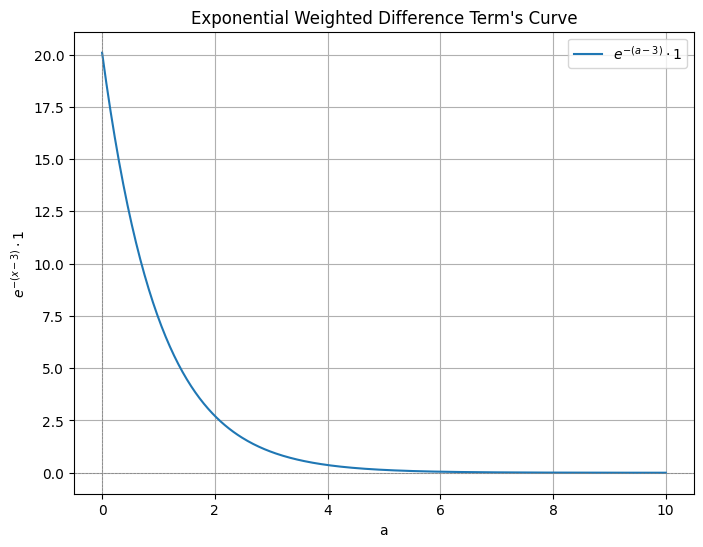
\includegraphics[width=0.75\linewidth]{resources/example exponential function.png}
    \caption{Exponential Weighted Difference Curve}
    \label{fig:example-exp-func-graph}
\end{figure}

The main challenge for the research problem in this thesis is finding
appropriate functions to evaluate the qualitative features to a numeric
value.

As identified in previous sections, criteria for evaluation in this work
are as follows

\subsubsection{Service set and performance
criteria}\label{service-set-and-performance-criteria}

We can define the service set and performance criteria as follows:

\begin{itemize}
\tightlist
\item
  \textbf{Service set (\(S\)):} (EKS, AKS, GKE, OCP)
\item
  \textbf{Performance criteria (\(C\)):} (Security, Costs, Maximum nodes
  in a cluster, Storage Provisioning, CNIs, Monitoring and Logging)
\end{itemize}

\section{Performance evaluation
functions}\label{performance-evaluation-functions}

The performance evaluation functions will determine how the score for
each criterion in set \(C\) is calculated. The function for each
criterion is defined as follow:

\subsection{Security}\label{security}

For all distribution, the security features are examined from a
\emph{functional} perspective. In other words, the following question is
evaluated: ``What is the output of this feature?''. Then, for each
distribution, count how many of the features/functions can be performed.

\subsection{Cost}\label{cost}

As mentioned in the section on managed Kubernetes, the costs for public
cloud services are publicly available and are often published on the
provider's website. For EKS, AKS, and GKE, the following parameters are
used to provide a standardised estimate for the cluster's management
fee:

\begin{itemize}
\tightlist
\item
  \textbf{Region:} Northern Europe (Stockholm, Helsinki if not available). This aims to make the
  evaluation more relevant to Nokia and Finnish businesses.
\item
  \textbf{Number of Clusters:} 1
\item
  \textbf{Type of Support/Support License Agreement (SLA):} The most
  extensive option. As stated in the CNCF Annual Survey 2023
  \cite{CNCFAnnualSurvey2024}, complexity is still the second most
  challenging problem for container operations. Thus, an extensive
  degree of support aims to reflect the practical needs of organisations
  when adopting these services.
\end{itemize}

Public cloud services often use the number of vCPUs as the criteria for
management cost calculation
\cite{RedHatOpenShiftc,PricingGoogleKubernetes}. In this evaluation, we
look at a standard cluster with 3 worker nodes, each with 20 vCPUs. The
full list of VM specifications are as follows:

\begin{itemize}
\tightlist
\item
  16 vCPUs
\item
  64 GB RAM
\item
  1 TB SSD
\item
  Up to 10 Gigabit network bandwidth
\end{itemize}

From these specifications, the monthly cost of operation is computed
based on the available information on the provider's website.

\subsection{Maximum nodes in a cluster}\label{maximum-nodes-in-a-cluster}

The Maximum number of nodes in a cluster is obtained through the
official documentation
\cite{Chapter4Planninga,KnownLimitsService,nickomangLimitsResourcesSKUs2024,QuotasLimitsGoogle}.
This is the maximum supported nodes in a single cluster. In the case of
GKE, while it is theoretically possible to increase the limit to 65,000
nodes, this requires special conditions and configurations. In addition,
special arrangements with GKE support is also required. Thus, the 5,000
nodes limit is used instead. This is also the limit that was used by
Truyen et al.~\cite{truyenManagingFeatureCompatibility2020}.

\subsection{Storage Provisioning, CNIs, and Monitoring and
Logging}\label{storage-provisioning-cnis-and-monitoring-and-logging}

For each criterion, the total number of supported options for that
underlying operation is determined from the provider's documentation and used as the evaluation points. 

\section{Result Normalisation}\label{result-normalisation}

As discussed by Rehman et al.~\cite{5976164}, the performance
measurement functions' result should be normalised to a unified range. A
min-max normalisation is performed on all resulting output above to
achieve a score on a scale from 0 to 5. The normalisation formula can be
found below:

\[
   \text{Normalized Value} = 5 \times \frac{x - \text{min}(x)}{\text{max}(x) - \text{min}(x)}
\]

\section{Adjustable parameters}\label{adjustable-parameters}

The other parameters for the Rehman framework used in this evaluation
are listed below:

\begin{enumerate}
\def\labelenumi{\arabic{enumi}.}
\tightlist
\item
  \textbf{User requirement criteria (\(R\)):} 0
\item
  \textbf{User priority weights (\(W\)):}

  \begin{itemize}
  \tightlist
  \item
    \textbf{Security:} 50
  \item
    \textbf{Costs:} 10
  \item
    \textbf{Maximum nodes:} 10
  \item
    \textbf{Storage provisioning:} 10
  \item
    \textbf{CNIs:} 10
  \item
    \textbf{Moniroting and Logging:} 10
  \end{itemize}
\end{enumerate}

The minimum requirements depend on the organisation's requirements.
In this case, since the evaluation does not cater to a single
organisation, there is no minimum requirement and the minimum
requirements are left as 0.

Regarding the weights, security is the key evaluation factor, as
discussed in the section \ref{chap:evaluation-criteria}. Therefore, a large weight value is
assigned to security. Each of the other features, on the other hand, get
assigned an equal portion of the remaining weight value.

These parameters can be adjusted appropriately to fit the organisation
requirements and priorities if needed.

\section{Result Compilation}\label{result-compilation}

From all parameters defined above, it is possible to compute the service
descriptor vector (\(D_i\)) and the decision matrix (\(A\)). Finally,
the decisision matrix is transformed into the EWD vector using the following formula. This vector
contains the resulting score of all the distributions evaluated, taking
into account all the mentioned factors. The scores provide insights
into how suitable each distribution is for enterprise use-cases based on
the given hypothetical set of parameters.

\chapter{Findings}

\section{Security Evaluation}

The features are identified from the official documentation of the selected services \cite{SecurityComplianceRed,SecurityOverview|,miwithroConceptsSecurityAzure2024,SecurityAmazonEKS}. For each feature, the functional question of "What is the output of this feature?" is evaluated. Through reviewing the official documentation of the selected vendors, 41 security features were identified and listed in table \ref{tab:feature_overview} in the Appendix. The corresponding feature support status is also identified in table \ref{tab:feature_support}.

The total number of supported feature by each distribution and the normalised score can be seen from table \ref{tab:feature-score}

\begin{table}[!ht]
    \centering
    \begin{tabular}{|p{4cm}|p{2cm}|p{2cm}|p{2cm}|p{2cm}|} % Set fixed widths for columns
    \hline
         & EKS & AKS & GKE & OCP \\ \hline
        Distribution Security Feature Count& 30& 33& 35& 33\\ \hline
 Distribution Security Feature Count (Normalised)& 1& 3& 5&3\\\hline
    \end{tabular}
    \caption{Cost Analysis Results} 
    \label{tab:feature-score}
\end{table}

\section{Cost Analysis}

With the specifications mentioned in the methodology section and the pricing information from the providers, the following costs are calculated \cite{CreateEstimateConfigure,PricingAzureKubernetes,GoogleCloudPricing,RedHatOpenShiftd}:
\begin{table}[!ht]
    \centering
    \begin{tabular}{|p{4cm}|p{2cm}|p{2cm}|p{2cm}|p{2cm}|} % Set fixed widths for columns
    \hline
         & EKS & AKS & GKE & OCP \\ \hline
        Management Cost & 73 & 72 & 288.03 & 500 \\ \hline
        Infrastructure Cost & 1535.78 & 1867.06 & 2541.97 & 2541.97 \\ \hline
        Total Cost & 1608.78 & 1939.06 & 2830 & 3041.97 \\ \hline
        Maximum Cost Difference & 1433.19 & 1102.91 & 211.97 & 0 \\ \hline
        Maximum Cost Differences (Normalised) & 5 & 4.078 & 1.592 & 1 \\ \hline
    \end{tabular}
    \caption{Cost Analysis Results} 
    \label{tab:cost-analysis}
\end{table}

\section{Fundamental Features Evaluation}

From the documentation, the followings were identified:

\textbf{Maximum Nodes per Cluster}

\begin{itemize}
\tightlist
\item
  EKS: 5,000 \cite{KnownLimitsService}
\item
  AKS: 5,000  \cite{nickomangLimitsResourcesSKUs2024}
\item
  GKE: 5,000 \cite{QuotasLimitsGoogle}
\item
  OCP: 2,000  \cite{Chapter4Planning}
\end{itemize}



\textbf{Storage:}

\begin{itemize}
\tightlist
\item
  EKS: 4 options supported
  S3 \cite{StoreApplicationData}
\item
     AKS: 6 options supported \cite{tamramConceptsStorageAzure2024}
\item
  GKE: 8 options supported \cite{StorageGKEClusters} 
\item
  OCP: 13 options supported \cite{UnderstandingPersistentStorage} 
\end{itemize}

\textbf{CNIs:}

\begin{itemize}
\tightlist
\item
  EKS: 5 CNIs supported \cite{AlternateCNIPlugins}
\item
  AKS: 4 CNIs supported \cite{schaffererinConceptsCNINetworking2024}
\item
  GKE: 4 CNIs supported \cite{NetworkOverviewGooglea}
\item
  OCP: 6 CNIs supported \cite{CertifiedOpenShiftCNI2024}
\end{itemize}

\textbf{Application Monitoring and Logging:}

\begin{itemize}
\tightlist
\item
  EKS: 1 option, Amazon Cloud Watch \cite{MonitorYourCluster}
\item
  AKS: 1 option, Azure Monitor \cite{martinekuanMonitorMicroservicesApplication}
\item
  GKE: 1 option, GKE logging agent \cite{GKELogsGoogle} 
\item
  OCP: 1 option, Loki Stack \cite{Logging60Logging}
\end{itemize}

The normalised score for this section can be seen below:

\begin{table}[!ht]
    \centering
    \begin{tabular}{|p{4cm}|p{2cm}|p{2cm}|p{2cm}|p{2cm}|} % Set fixed widths for columns
    \hline
         & EKS & AKS & GKE & OCP \\ \hline
        Supported Storage Provisioning Options & 4& 6& 8& 13\\ \hline
        Supported Storage Provisioning Options (Normalised)& 1& 1.89& 2.78& 5\\ \hline
        Supported CNI Options& 5& 4& 4& 6\\ \hline
        Supported CNI Options (Normalised)& 3& 1& 1& 5\\ \hline
        Supported Logging Options& 1& 1& 1& 1\\ \hline
 Supported Logging Options (Normalised)& 1& 1& 1&1\\\hline
 Maximum Nodes& 5000& 5000& 5000&2000\\\hline
 Maximum Nodes (Normalised)& 5& 5& 5&1\\\hline
    \end{tabular}
    \caption{Fundamental Features Analysis} 
    \label{tab:cost-analysis}
\end{table}

\section{EWD}

\begin{table}[!ht]
    \centering
    \begin{tabular}{|p{4cm}|p{2cm}|p{2cm}|p{2cm}|p{2cm}|} % Set fixed widths for columns
    \hline
         & EKS& AKS& GKE& OCP\\ \hline
        Normalised Security& 1.00& 3.00& 5.00& 3.00\\ \hline
        Normalised Cost& 5.00& 4.08& 1.59& 1.00\\ \hline
        Normalised Max Nodes& 5.00& 5.00& 5.00& 1.00\\ \hline
        Normalised Storage& 1.00& 1.89& 2.78& 5.00\\ \hline
        Normalised CNI& 3.00& 1.00& 1.00& 5.00\\ \hline
 Normalised Logging& 0.00& 0.00& 0.00&0.00\\\hline
 EWDs& 4.47& 4.23& 4.20&4.25\\\hline
    \end{tabular}
    \caption{Exponential Weighted Difference Results} 
    \label{tab:cost-analysis}
\end{table}

\chapter{Discussion}

Based on the findings. It appears that with the given parameters, GKE seems to be the most suitable distribution for the particular use-case evaluated. This can be largely attributed to the fact that GKE possess a higher amount of security features compare to the other distributions evaluated in this thesis.

The criteria were chosen based on the perceived interests of companies and organisations displayed in the reviewed surveys. However, these findings do not meant to be prescriptive for all use-cases. As discussed, the framework proposed by Rehman et al. \cite{5976164} can be customised to fit the needs of an organisation on a case-by-case basis.

With a different set of criteria, evaluation functions, weights, and user requirements, it is possible to arrive at a dissimilar ranking of distributions. Of course, this potential for customisation is one of the benefit of the chosen framework.

\chapter{Conclusion}

This thesis examines four major managed Kubernetes distributions and compare them in terms of security, costs, and other fundamental features. The qualitative features are quantified and combined to reach the final evaluation scores of the distributions Based on the scores, a clear ranking of distributions were provided.

In addition, utilising the framework proposed by Rehman et al. \cite{5976164}, a structured procedure for multi-criteria cloud service selection was demonstrated. This work evaluated the distribution on a general level based on projected industrial interests. However, the same process can be applied and customised to specific organisational needs to achieve more relevant results. Through a systematic examination of features, organisations can make informed decisions that align closely with their requirements.

Given the evidenced demand for managed Kubernetes, there is potential for further research in this domain. Future work could explore, for instance, a broader array of metrics than those reviewed in this thesis. Due to the limited resource, only a handful of selected qualitative features were selected for assessment. However, it is possible to include quantiative metrics such as computational performance (in terms of CPU, memory, disk I/O, networking, etc.) to achieve a more comprehensive analysis.


















%%  LIITTEET  ------------------------------------------

% \appendix
% \chapter{Ut purus elit}

% Lorem ipsum dolor sit amet, consectetuer adipiscing elit. Ut purus
% elit, vestibulum ut, placerat ac, adipiscing vitae, felis. Curabitur
% dictum gravida mauris. Nam arcu libero, nonummy eget, consectetuer id,
% vulputate a, magna. Donec vehicula augue eu neque. Pellentesque
% habitant morbi tristique senectus et netus et malesuada fames ac
% turpis egestas. Mauris ut leo. Cras viverra metus rhoncus sem. Nulla
% et lectus vestibulum urna fringilla ultrices. Phasellus eu tellus sit
% amet tortor gravida placerat. Integer sapien est, iaculis in, pretium
% quis, viverra ac, nunc. Praesent eget sem vel leo ultrices
% bibendum. Aenean faucibus. Morbi dolor nulla, malesuada eu, pulvinar
% at, mollis ac, nulla. Curabitur auctor semper nulla.  Donec varius
% orci eget risus. Duis nibh mi, congue eu, accumsan eleifend, sagittis
% quis, diam. Duis eget orci sit amet orci dignissim rutrum.

% Nam dui ligula, fringilla a, euismod sodales, sollicitudin vel,
% wisi. Morbi auctor lorem non justo. Nam lacus libero, pretium at,
% lobortis vitae, ultricies et, tellus. Donec aliquet, tortor sed
% accumsan bibendum, erat ligula aliquet magna, vitae ornare odio metus
% a mi. Morbi ac orci et nisl hendrerit mollis. Suspendisse ut
% massa. Cras nec ante. Pellentesque a nulla.  Cum sociis natoque
% penatibus et magnis dis parturient montes, nascetur ridiculus
% mus. Aliquam tincidunt urna. Nulla ullamcorper vestibulum
% turpis. Pellentesque cursus luctus mauris.

% \section{Fusce mauris}

% Fusce mauris. Vestibulum luctus nibh at lectus. Sed bibendum, nulla a
% faucibus semper, leo velit ultricies tellus, ac venenatis arcu wisi
% vel nisl.  Vestibulum diam. Aliquam pellentesque, augue quis sagittis
% posuere, turpis lacus congue quam, in hendrerit risus eros eget
% felis. Maecenas eget erat in sapien mattis porttitor. Vestibulum
% porttitor. Nulla facilisi.  Sed a turpis eu lacus commodo
% facilisis. Morbi fringilla, wisi in dignissim interdum, justo lectus
% sagittis dui, et vehicula libero dui cursus dui. Mauris tempor ligula
% sed lacus. Duis cursus enim ut augue. Cras ac magna.  Cras
% nulla. Nulla egestas. Curabitur a leo. Quisque egestas wisi eget
% nunc. Nam feugiat lacus vel est. Curabitur consectetuer.


\renewcommand{\bibname}{References (IEEE)}
\printbibliography
% \bibliography{references.bib}

\chapter{Appendix}

\begin{longtable}{p{0.35\linewidth} p{0.65\linewidth}} % Adjusted column widths
\caption{Feature Overview and Descriptions} \label{tab:feature_overview} \\

\toprule
\textbf{Feature Name} & \textbf{Description} \\
\midrule
\endfirsthead % Header for the first page

\toprule
\textbf{Feature Name} & \textbf{Description} \\
\midrule
\endhead % Header for subsequent pages

\bottomrule
\endfoot % Footer for all but last page

\endlastfoot % Footer for the last page

\textbf{Kubernetes Role-Based Access Control (RBAC) Support} & Provides fine-grained access control by defining permissions for users and groups within Kubernetes clusters. \\
\hline
\textbf{Integration of Cloud IAM with Kubernetes RBAC} & Maps cloud provider IAM entities to Kubernetes RBAC roles for unified access control across cloud and cluster resources. \\
\hline
\textbf{Kubernetes Service Account Support} & Assigns permissions to pods via service accounts, controlling API resource access within the cluster. \\
\hline
\textbf{IAM Roles for Service Accounts / Workload Identity Federation} & Integrates service accounts with cloud IAM roles, allowing secure access to cloud resources from workloads. \\
\hline
\textbf{Cluster Authentication and Authorization} & Manages who can access the cluster (authentication) and what actions they can perform (authorization). \\
\hline
\textbf{Linux Capabilities Management and Security Profiles} & Controls Linux capabilities for containers and manages security profiles like Seccomp and SELinux for enhanced container security. \\
\hline
\textbf{Network Policies} & Restricts pod-to-pod communication using labels or IP ranges, managing traffic within the cluster. \\
\hline
\textbf{Pod Security Policies / Admission Controllers / Security Context Constraints} & Enforces security settings at the pod level, controlling privileges and applying security contexts. \\
\hline
\textbf{Node Affinity and Taints/Tolerations} & Schedules pods to specific nodes, providing workload isolation and optimized resource utilization. \\
\hline
\textbf{TLS/SSL Support and Encryption} & Ensures secure communication by enforcing TLS protocols and managing SSL certificates for cluster components. \\
\hline
\textbf{Kubernetes Secrets Encryption / Data Encryption at Rest} & Encrypts sensitive data stored in secrets or etcd, protecting information at rest within the cluster. \\
\hline
\textbf{Vulnerability Scanning and Compliance Benchmarking} & Scans cluster configurations and container images for vulnerabilities, ensuring compliance with security standards like CIS benchmarks. \\
\hline
\textbf{Private Clusters / VPC Integration} & Limits API server access using virtual networks, enhancing security by restricting public exposure and integrating with Virtual Private Clouds (VPCs). \\
\hline
\textbf{Node and Network Security Groups} & Defines network-level access controls using security groups or network policies, controlling traffic to and from nodes and control plane components. \\
\hline
\textbf{Image Integrity Enforcement / Binary Authorization} & Ensures that only trusted container images are deployed through signature verification and policy compliance. \\
\hline
\textbf{Container-Optimized Operating Systems} & Uses hardened OS images for nodes with enhanced security features like read-only filesystems and minimized user accounts. \\
\hline
\textbf{Workload Sandbox / Kernel-Level Isolation / Confidential Containers} & Provides additional isolation for workloads using sandboxing technologies or confidential computing to protect data in use. \\
\hline
\textbf{Audit Logging} & Records cluster activities and API calls for auditing and compliance purposes, helping detect unauthorized actions. \\
\hline
\textbf{Access Control at Network Layer} & Implements network-level access controls using firewalls, security groups, or network policies to manage traffic flow. \\
\hline
\textbf{Kubernetes Node Authorization} & Manages authorization for Kubernetes nodes, determining what actions nodes can perform within the cluster. \\
\hline
\textbf{Policy-as-Code Support} & Allows policies and access controls to be defined and managed as code, enabling version control and automation. \\
\hline
\textbf{Separate Public and Private IP Subnets} & Isolates public-facing services from internal cluster components by segregating network subnets, enhancing security. \\
\hline
\textbf{Signed API Requests} & Requires API requests to be signed with credentials, ensuring the authenticity and integrity of client requests. \\
\hline
\textbf{Automatic Least-Privilege Determination} & Automatically identifies the minimal required permissions for applications, facilitating the principle of least privilege. \\
\hline
\textbf{Credential and Certificate Rotation} & Automates the rotation of credentials and SSL certificates to maintain security over time. \\
\hline
\textbf{Access Control for Support Personnel} & Provides mechanisms like just-in-time access roles for support staff, granting temporary and limited access to cluster resources. \\
\hline
\textbf{Image Build Security and Vulnerability Scanning} & Performs static analysis and vulnerability scanning of container images before deployment to ensure they meet security standards. \\
\hline
\textbf{Modified File Monitoring} & Continuously monitors file integrity on cluster nodes, logging any unauthorized modifications. \\
\hline
\textbf{Virtual Trusted Platform Module (vTPM) Support} & Uses virtual TPMs to provide hardware-based security features like secure key storage and remote attestation. \\
\hline
\textbf{ETCD Encryption} & Encrypts data stored in the etcd key-value store, securing cluster state information and protecting against unauthorized access. \\
\hline
\textbf{Automated Compliance Scanning and Remediation Suggestions} & Automatically scans for compliance with security standards and provides recommendations for remediation. \\
\hline
\textbf{Automatic Image Signature Verification} & Verifies container image signatures upon deployment to ensure they come from trusted sources. \\
\hline
\textbf{Automation of Tang Server Deployment for Disk Encryption} & Automates network-bound disk encryption using Tang servers, providing automatic unlocking of encrypted volumes. \\
\hline
\textbf{TLS Security Profile Configuration} & Allows customization of TLS settings and ciphers used by cluster components to meet specific security requirements. \\
\hline
\textbf{Shielded Nodes} & Provides node-level security features like secure boot and integrity monitoring to protect against boot-time attacks. \\
\hline
\textbf{Admission Controllers} & Uses admission plugins to enforce policies on API requests before they are persisted in the cluster. \\
\hline
\textbf{Kernel-Level Security Features} & Employs security features like AppArmor, Seccomp, and SELinux to restrict the actions that containers can perform. \\
\hline
\textbf{Support for Confidential Containers} & Provides containers that encrypt data in use, preventing access to the data by the host OS or hypervisor. \\
\hline
\textbf{Segmented Network / Multitenancy Support} & Segments network traffic within the cluster to isolate users, teams, applications, and environments. \\
\hline
\textbf{Managing Linux Capabilities and Security Profiles Cluster-wide} & Manages Linux security profiles across nodes for consistent application and enhanced security. \\
\hline
\textbf{Filtering Traffic with kube-proxy} & Uses kube-proxy to filter traffic based on IP addresses and ports, controlling service access within the cluster. \\

\end{longtable}


\begin{longtable}{p{0.74\linewidth} p{0.06\linewidth} p{0.06\linewidth} p{0.06\linewidth} p{0.06\linewidth}}
\caption{Feature Support Status} \label{tab:feature_support} \\

\toprule
\textbf{Feature Name} & \textbf{EKS} & \textbf{AKS} & \textbf{GKE} & \textbf{OCP} \\
\midrule
\endfirsthead

\toprule
\textbf{Feature Name} & \textbf{EKS} & \textbf{AKS} & \textbf{GKE} & \textbf{OCP} \\
\midrule
\endhead

\bottomrule
\endfoot

\endlastfoot
\textbf{1. Kubernetes Role-Based Access Control (RBAC) Support} & Yes &
Yes & Yes & Yes \\
\textbf{2. Integration of Cloud IAM with Kubernetes RBAC} & Yes & Yes &
Yes & Yes \\
\textbf{3. Kubernetes Service Account Support} & Yes & Yes & Yes &
Yes \\
\textbf{4. IAM Roles for Service Accounts / Workload Identity
Federation} & Yes & Yes & Yes & \small{Partial} \\
\textbf{5. Cluster Authentication and Authorization} & Yes & Yes & Yes &
Yes \\
\textbf{6. Linux Capabilities Management and Security Profiles} & Yes &
Yes & Yes & Yes \\
\textbf{7. Network Policies} & Yes & Yes & Yes & Yes \\
\textbf{8. Pod Security Policies / Admission Controllers / Security
Context Constraints} & Yes & Yes & Yes & Yes \\
\textbf{9. Node Affinity and Taints/Tolerations} & Yes & Yes & Yes &
Yes \\
\textbf{10. TLS/SSL Support and Encryption} & Yes & Yes & Yes & Yes \\
\textbf{11. Kubernetes Secrets Encryption / Data Encryption at Rest} &
Yes & Yes & Yes & Yes \\
\textbf{12. Vulnerability Scanning and Compliance Benchmarking} &
\small{Partial} & Yes & Yes & Yes \\
\textbf{13. Private Clusters / VPC Integration} & Yes & Yes & Yes &
Yes \\
\textbf{14. Node and Network Security Groups} & Yes & Yes & Yes &
\small{Partial} \\
\textbf{15. Image Integrity Enforcement / Binary Authorization} &
\small{Partial} & Yes & Yes & Yes \\
\textbf{16. Container-Optimized Operating Systems} & Yes & Yes & Yes &
Yes \\
\textbf{17. Workload Sandbox / Kernel-Level Isolation / Confidential
Containers} & \small{Partial} & Yes & Yes & \small{Partial} \\
\textbf{18. Audit Logging} & Yes & Yes & Yes & Yes \\
\textbf{19. Access Control at Network Layer} & Yes & Yes & Yes & Yes \\
\textbf{20. Kubernetes Node Authorization} & Yes & Yes & Yes & Yes \\
\textbf{21. Policy-as-Code Support} & Yes & Yes & Yes & Yes \\
\textbf{22. Separate Public and Private IP Subnets} & Yes & Yes & Yes &
Yes \\
\textbf{23. Signed API Requests} & Yes & No & No & No \\
\textbf{24. Automatic Least-Privilege Determination} & Yes & No & No &
No \\
\textbf{25. Credential and Certificate Rotation} & Yes & Yes & Yes &
Yes \\
\textbf{26. Access Control for Support Personnel} & No & Yes & No &
No \\
\textbf{27. Image Build Security and Vulnerability Scanning} & \small{Partial} &
Yes & Yes & Yes \\
\textbf{28. Modified File Monitoring} & No & No & No & Yes \\
\textbf{29. Virtual Trusted Platform Module (vTPM) Support} & No & No &
Yes & No \\
\textbf{30. ETCD Encryption} & Yes & Yes & Yes & Yes \\
\textbf{31. Automated Compliance Scanning and Remediation Suggestions} &
\small{Partial} & Yes & Yes & Yes \\
\textbf{32. Automatic Image Signature Verification} & \small{Partial} & Yes &
Yes & Yes \\
\textbf{33. Automation of Tang Server Deployment for Disk Encryption} &
No & No & No & Yes \\
\textbf{34. TLS Security Profile Configuration} & \small{Partial} & \small{Partial} &
\small{Partial} & Yes \\
\textbf{35. Shielded Nodes} & No & No & Yes & No \\
\textbf{36. Admission Controllers} & Yes & Yes & Yes & Yes \\
\textbf{37. Kernel-Level Security Features} & Yes & Yes & Yes & Yes \\
\textbf{38. Support for Confidential Containers} & No & Yes & Yes &
\small{Partial} \\
\textbf{39. Segmented Network / Multitenancy Support} & Yes & Yes & Yes
& Yes \\
\textbf{40. Managing Linux Capabilities and Security Profiles
Cluster-wide} & \small{Partial} & \small{Partial} & \small{Partial} & Yes \\
\textbf{41. Filtering Traffic with kube-proxy} & No & No & Yes & No \\
\end{longtable}


\textbf{Legend:}

\begin{itemize}
\tightlist
\item
  \textbf{Yes}: The platform supports the feature.
\item
  \textbf{Partial}: The platform offers limited support or requires
  additional configuration/tools.
\item
  \textbf{No}: The platform does not support the feature.
\end{itemize}


\end{document}
